% Options for packages loaded elsewhere
\PassOptionsToPackage{unicode}{hyperref}
\PassOptionsToPackage{hyphens}{url}
%
\documentclass[
]{article}
\usepackage{lmodern}
\usepackage{amsmath}
\usepackage{ifxetex,ifluatex}
\ifnum 0\ifxetex 1\fi\ifluatex 1\fi=0 % if pdftex
  \usepackage[T1]{fontenc}
  \usepackage[utf8]{inputenc}
  \usepackage{textcomp} % provide euro and other symbols
  \usepackage{amssymb}
\else % if luatex or xetex
  \usepackage{unicode-math}
  \defaultfontfeatures{Scale=MatchLowercase}
  \defaultfontfeatures[\rmfamily]{Ligatures=TeX,Scale=1}
\fi
% Use upquote if available, for straight quotes in verbatim environments
\IfFileExists{upquote.sty}{\usepackage{upquote}}{}
\IfFileExists{microtype.sty}{% use microtype if available
  \usepackage[]{microtype}
  \UseMicrotypeSet[protrusion]{basicmath} % disable protrusion for tt fonts
}{}
\makeatletter
\@ifundefined{KOMAClassName}{% if non-KOMA class
  \IfFileExists{parskip.sty}{%
    \usepackage{parskip}
  }{% else
    \setlength{\parindent}{0pt}
    \setlength{\parskip}{6pt plus 2pt minus 1pt}}
}{% if KOMA class
  \KOMAoptions{parskip=half}}
\makeatother
\usepackage{xcolor}
\IfFileExists{xurl.sty}{\usepackage{xurl}}{} % add URL line breaks if available
\IfFileExists{bookmark.sty}{\usepackage{bookmark}}{\usepackage{hyperref}}
\hypersetup{
  pdftitle={Application results},
  pdfauthor={Nutcha Wattanachit},
  hidelinks,
  pdfcreator={LaTeX via pandoc}}
\urlstyle{same} % disable monospaced font for URLs
\usepackage[margin=1in]{geometry}
\usepackage{graphicx}
\makeatletter
\def\maxwidth{\ifdim\Gin@nat@width>\linewidth\linewidth\else\Gin@nat@width\fi}
\def\maxheight{\ifdim\Gin@nat@height>\textheight\textheight\else\Gin@nat@height\fi}
\makeatother
% Scale images if necessary, so that they will not overflow the page
% margins by default, and it is still possible to overwrite the defaults
% using explicit options in \includegraphics[width, height, ...]{}
\setkeys{Gin}{width=\maxwidth,height=\maxheight,keepaspectratio}
% Set default figure placement to htbp
\makeatletter
\def\fps@figure{htbp}
\makeatother
\setlength{\emergencystretch}{3em} % prevent overfull lines
\providecommand{\tightlist}{%
  \setlength{\itemsep}{0pt}\setlength{\parskip}{0pt}}
\setcounter{secnumdepth}{-\maxdimen} % remove section numbering
\usepackage{amsmath}
\usepackage{tabularx}
\usepackage{hyperref}
\usepackage{multicol}
\usepackage{longtable}
\usepackage{array}
\usepackage{multirow}
\usepackage{wrapfig}
\usepackage{float}
\usepackage{colortbl}
\usepackage{pdflscape}
\usepackage{booktabs}
\usepackage{tabu}
\usepackage{threeparttable}
\usepackage{threeparttablex}
\usepackage{makecell}
\usepackage{xcolor}
\usepackage{booktabs}
\usepackage{longtable}
\usepackage{array}
\usepackage{multirow}
\usepackage{wrapfig}
\usepackage{float}
\usepackage{colortbl}
\usepackage{pdflscape}
\usepackage{tabu}
\usepackage{threeparttable}
\usepackage{threeparttablex}
\usepackage[normalem]{ulem}
\usepackage{makecell}
\usepackage{xcolor}
\ifluatex
  \usepackage{selnolig}  % disable illegal ligatures
\fi

\title{Application results}
\author{Nutcha Wattanachit}
\date{06/29/2021}

\begin{document}
\maketitle

We compare 1) the equally-weighted ensemble (EW), 2) the traditional
linear pool (TLP), 3) the beta-transform linear pool (BLP), 4) the
equally-weighted beta-transform linear pool, 5) the finite beta mixture
6) the finite beta mixture with equally-weighted component forecasts in
the simulation studies and in the application of influenza forecasting.
For both beta mixture approaches, the number of mixing beta components
are \(K=2,3,4,5\).

\hypertarget{methods}{%
\section{Methods}\label{methods}}

Let \(f_1,...,f_M\) be predictive density forecasts from \(M\) component
forecasting models, the ensemble methods combine the component
forecasting models as follows

\hypertarget{equally-weighted-ensemble-ew}{%
\subsection{Equally-weighted ensemble
(EW)}\label{equally-weighted-ensemble-ew}}

The equally-weighted ensemble combines the component forecasting models
with the aggregation predictive distribution function

\begin{align}
f_{\text{EW}}(y)=\sum_{m=1}^M \frac{1}{M}f_m(y).
\end{align}

\hypertarget{traditional-linear-pool-tlp}{%
\subsection{Traditional linear pool
(TLP)}\label{traditional-linear-pool-tlp}}

The TLP finds a set of optimal nonnegative weights \(w_i\) that maximize
the likelihood of the aggregation predictive distribution function

\begin{align}
f_{\text{TLP}}(y)=\sum_{m=1}^M w_mf_m(y),
\end{align}

where \(\sum_{m=1}^M w_m=1\). The TLP is underdispersed when the
component models are probabilistically calibrated.

\hypertarget{beta-transform-linear-pool-blp}{%
\subsection{Beta-transform linear pool
(BLP)}\label{beta-transform-linear-pool-blp}}

The BLP applies a beta transform on the combined predictive cumulative
distribution function

\begin{align}
F_{\text{BLP}}(y)=B_{\alpha,\beta}\Big(\sum_{m=1}^M w_m F_m(y)\Big),
\end{align}

Specifically, the BLP finds the transformation parameters
\(\alpha,\beta > 0\), and a set of nonnegative weights \(w_m\) that
maximize the likelihood of the aggregated predictive distribution
function

\begin{align}
f_{\text{BLP}}(y)=\Big(\sum_{m=1}^M w_mf_m(y)\Big)b_{\alpha,\beta}\Big(\sum_{m=1}^M w_m F_m(y)\Big),
\end{align}

where \(b_{\alpha,\beta}\) denotes the beta density and
\(\sum_{m=1}^M w_m=1\).

\hypertarget{equally-weighted-beta-transform-linear-pool-ew-blp}{%
\subsection{Equally-weighted beta-transform linear pool
(EW-BLP)}\label{equally-weighted-beta-transform-linear-pool-ew-blp}}

The EW-BLP applies a beta transform on the equally-weighted ensemble and
has the predictive cumulative distribution function

\begin{align}
F_{\text{EW-BLP}}(y)=B_{\alpha,\beta}\Big(\sum_{m=1}^M \frac{1}{M} F_m(y)\Big),
\end{align}

The EW-BLP finds the transformation parameters \(\alpha,\beta > 0\) that
maximize the likelihood of the aggregated predictive distribution
function

\begin{align}
f_{\text{EW-BLP}}(y)=\Big(\sum_{m=1}^M w_mf_m(y)\Big)b_{\alpha,\beta}\Big(\sum_{m=1}^M \frac{1}{M} F_m(y)\Big).
\end{align}

\hypertarget{finite-beta-mixture-textbm_k}{%
\subsection{\texorpdfstring{Finite beta mixture
(\(\text{BM}_k\))}{Finite beta mixture (\textbackslash text\{BM\}\_k)}}\label{finite-beta-mixture-textbm_k}}

The \(\text{BM}_k\) extends the BLP method by using a finite beta
mixture combination formula

\begin{align}
F_{\text{BM}_k}(y)=\sum_{k=1}^K w_kB_{\alpha,\beta}\Big(\sum_{m=1}^M \omega_{km} F_m(y)\Big),
\end{align}

where the vector \(w_1,..., w_K\) comprises the beta mixture weights,
\(\alpha_1,..., \alpha_K\) and \(\beta_1,..., \beta_K\) are beta
calibration parameters, and for each beta component
\(\boldsymbol{\omega}_k=(\omega_{k1},..., \omega_{kM})\) comprises the
beta component-specific set of component model weights. The pdf
representation of the method is

\begin{align}
f_{\text{BM}_k}(y)=\sum_{k=1}^K w_k(\sum_{m=1}^M \omega_{km} f_m(y)\Big)b_{\alpha,\beta}\Big(\sum_{m=1}^M \omega_{km} F_m(y)\Big).
\end{align}

\hypertarget{finite-beta-mixture-with-equally-weighted-ensemble-textew-bm_k}{%
\subsection{\texorpdfstring{Finite beta mixture with equally weighted
ensemble
(\(\text{EW-BM}_k\))}{Finite beta mixture with equally weighted ensemble (\textbackslash text\{EW-BM\}\_k)}}\label{finite-beta-mixture-with-equally-weighted-ensemble-textew-bm_k}}

The \(\text{EW-BM}_k\) uses a finite beta mixture combination formula to
combine an equally-weighted ensemble as follows

\begin{align}
F_{\text{EW-BM}_k}(y)=\sum_{k=1}^K w_kB_{\alpha,\beta}\Big(\sum_{m=1}^M \frac{1}{M} F_m(y)\Big),
\end{align}

where the vector \(w_1,..., w_K\) comprises the beta mixture weights and
\(\alpha_1,..., \alpha_K\) and \(\beta_1,..., \beta_K\) are beta
calibration parameters.

\begin{align}
f_{\text{EW-BM}_k}(y)=\sum_{k=1}^K w_k(\sum_{m=1}^M \frac{1}{M} f_m(y)\Big)b_{\alpha,\beta}\Big(\sum_{m=1}^M \frac{1}{M} F_m(y)\Big).
\end{align}

\hypertarget{cross-validation-and-training-process}{%
\section{Cross Validation and Training
Process}\label{cross-validation-and-training-process}}

The 2016/2017, 2017/2018, 2018/2019 seasons are selected as the test
seasons. For the mixture methods, \(\text{BMC}_k\) and
\(\text{EW-BMC}_k\), the leave-one-season-out cross validation is used
to select the number of beta mixture component \(k\). For each test
season, all the seasons preceding the test season are used for the
leave-one-season-out cross validation (i.e., if there are \(N\) seasons
up until the test season, then \(N-1\) seasons are used in the
leave-one-season-out cross validation with \(N-2\) seasons as training
seasons and each one of the \(N-1\) seasons is the validation season).
The mean validation log scores are calculated across all \(N-1\)
seasons, and one lowest \(k\) with the mean validation log scores within
one standard deviation of all methods' mean validation log scores is
selected for \(\text{BMC}_k\) and \(\text{EW-BMC}_k\). We did not simply
pick the methods with lowest mean validation log scores in order to take
into account model complexity (a less complex model is preferred with
the mean validation log score is not much worse compared to a more
complex model).

The four methods (BLP, EW-BLP, selected \(\text{BMC}_k\), selected
\(\text{EW-BMC}_k\)) are trained all the seasons preceding each test
season and the mean log scores are calculated across all week,locations,
training seasons. For EW and TLP, the first does not need training and
we use the FSN-TW ensemble's estimated parameters for the latter. The
estimated parameters are applied to build the ensembles for the test
season and the mean log scores are calculated across all week and
locations for all three test seasons.

\hypertarget{log-scores}{%
\section{Log scores}\label{log-scores}}

\hypertarget{cross-validated-mean-log-scores-for-textbmc_k-and-textew-bmc_k}{%
\subsection{\texorpdfstring{Cross-validated mean log scores for
\(\text{BMC}_k\) and
\(\text{EW-BMC}_k\)}{Cross-validated mean log scores for \textbackslash text\{BMC\}\_k and \textbackslash text\{EW-BMC\}\_k}}\label{cross-validated-mean-log-scores-for-textbmc_k-and-textew-bmc_k}}

\begin{table}[H]

\caption{\label{tab:unnamed-chunk-2}Test season 2016/2017}
\centering
\begin{tabular}[t]{llrr}
\toprule
Target & Model Name & Mean train log score & Mean validation log score\\
\midrule
1 wk ahead & BMC2 & -2.432 & -2.495\\
1 wk ahead & BMC3 & -2.422 & -2.499\\
1 wk ahead & BMC4 & -2.416 & -2.497\\
1 wk ahead & BMC5 & -2.407 & -2.501\\
1 wk ahead & EW\_BMC2 & -2.494 & -2.500\\
1 wk ahead & EW\_BMC3 & -2.494 & -2.501\\
1 wk ahead & EW\_BMC4 & -2.494 & -2.502\\
1 wk ahead & EW\_BMC5 & -2.494 & -2.503\\
2 wk ahead & BMC2 & -2.674 & -2.744\\
2 wk ahead & BMC3 & -2.664 & -2.755\\
2 wk ahead & BMC4 & -2.653 & -2.758\\
2 wk ahead & BMC5 & -2.650 & -2.763\\
2 wk ahead & EW\_BMC2 & -2.747 & -2.763\\
2 wk ahead & EW\_BMC3 & -2.746 & -2.765\\
2 wk ahead & EW\_BMC4 & -2.745 & -2.767\\
2 wk ahead & EW\_BMC5 & -2.745 & -2.767\\
3 wk ahead & BMC2 & -2.837 & -2.945\\
3 wk ahead & BMC3 & -2.820 & -2.948\\
3 wk ahead & BMC4 & -2.813 & -2.953\\
3 wk ahead & BMC5 & -2.801 & -2.974\\
3 wk ahead & EW\_BMC2 & -2.898 & -2.916\\
3 wk ahead & EW\_BMC3 & -2.897 & -2.916\\
3 wk ahead & EW\_BMC4 & -2.897 & -2.917\\
3 wk ahead & EW\_BMC5 & -2.896 & -2.917\\
4 wk ahead & BMC2 & -2.952 & -3.077\\
4 wk ahead & BMC3 & -2.942 & -3.088\\
4 wk ahead & BMC4 & -2.930 & -3.103\\
4 wk ahead & BMC5 & -2.923 & -3.109\\
4 wk ahead & EW\_BMC2 & -3.018 & -3.033\\
4 wk ahead & EW\_BMC3 & -3.017 & -3.035\\
4 wk ahead & EW\_BMC4 & -3.016 & -3.036\\
4 wk ahead & EW\_BMC5 & -3.015 & -3.036\\
\bottomrule
\end{tabular}
\end{table}

\begin{itemize}
\item BMC2 and EM-BMC2 have the lowest mean validation log scores and are selected for training for all targets. 
\item For 1 and 2 week ahead targets, $\text{BMC}_k$ outperform $\text{EW-BMC}_k$ with the same $k$, but the reverse is true for 3 and 4 week ahead targets.
\item We start to see some evidence of overfitting in $\text{BMC}_k$ compared to $\text{EW-BMC}_k$ for 3 and 4 week ahead targets ($\text{BMC}_k$'s train log scores are higher, but the mean validation log scores are worse than $\text{EW-BMC}_k$'s).
\end{itemize}

\newpage

\begin{table}[H]

\caption{\label{tab:unnamed-chunk-3}Test season 2017/2018}
\centering
\begin{tabular}[t]{llrr}
\toprule
Target & Model Name & Mean train log score & Mean validation log score\\
\midrule
1 wk ahead & BMC2 & -2.450 & -2.495\\
1 wk ahead & BMC3 & -2.442 & -2.501\\
1 wk ahead & BMC4 & -2.435 & -2.502\\
1 wk ahead & BMC5 & -2.430 & -2.507\\
1 wk ahead & EW\_BMC2 & -2.509 & -2.514\\
1 wk ahead & EW\_BMC3 & -2.509 & -2.514\\
1 wk ahead & EW\_BMC4 & -2.509 & -2.514\\
1 wk ahead & EW\_BMC5 & -2.508 & -2.516\\
2 wk ahead & BMC2 & -2.697 & -2.755\\
2 wk ahead & BMC3 & -2.688 & -2.754\\
2 wk ahead & BMC4 & -2.680 & -2.763\\
2 wk ahead & BMC5 & -2.674 & -2.770\\
2 wk ahead & EW\_BMC2 & -2.767 & -2.780\\
2 wk ahead & EW\_BMC3 & -2.767 & -2.782\\
2 wk ahead & EW\_BMC4 & -2.766 & -2.782\\
2 wk ahead & EW\_BMC5 & -2.766 & -2.783\\
3 wk ahead & BMC2 & -2.869 & -2.957\\
3 wk ahead & BMC3 & -2.857 & -2.964\\
3 wk ahead & BMC4 & -2.846 & -2.970\\
3 wk ahead & BMC5 & -2.841 & -2.981\\
3 wk ahead & EW\_BMC2 & -2.929 & -2.944\\
3 wk ahead & EW\_BMC3 & -2.928 & -2.946\\
3 wk ahead & EW\_BMC4 & -2.927 & -2.947\\
3 wk ahead & EW\_BMC5 & -2.926 & -2.948\\
4 wk ahead & BMC2 & -2.986 & -3.093\\
4 wk ahead & BMC3 & -2.967 & -3.087\\
4 wk ahead & BMC4 & -2.960 & -3.105\\
4 wk ahead & BMC5 & -2.954 & -3.108\\
4 wk ahead & EW\_BMC2 & -3.045 & -3.062\\
4 wk ahead & EW\_BMC3 & -3.045 & -3.062\\
4 wk ahead & EW\_BMC4 & -3.042 & -3.062\\
4 wk ahead & EW\_BMC5 & -3.043 & -3.062\\
\bottomrule
\end{tabular}
\end{table}

\begin{itemize}
\item BMC2 and EM-BMC2 have the lowest mean validation log scores and are selected for training for all targets. 
\item For 1 and 2 week ahead targets, $\text{BMC}_k$ outperform $\text{EW-BMC}_k$ with the same $k$, but the reverse is true for 3 and 4 week ahead targets.
\item We start to see some evidence of overfitting in $\text{BMC}_k$ compared to $\text{EW-BMC}_k$ for 3 and 4 week ahead targets ($\text{BMC}_k$'s train log scores are higher, but the mean validation log scores are worse than $\text{EW-BMC}_k$'s).
\end{itemize}

\newpage

\begin{table}[H]

\caption{\label{tab:unnamed-chunk-4}Test season 2018/2019}
\centering
\begin{tabular}[t]{llrr}
\toprule
Target & Model Name & Mean train log score & Mean validation log score\\
\midrule
1 wk ahead & BMC2 & -2.474 & -2.512\\
1 wk ahead & BMC3 & -2.466 & -2.517\\
1 wk ahead & BMC4 & -2.460 & -2.525\\
1 wk ahead & BMC5 & -2.456 & -2.526\\
1 wk ahead & EW\_BMC2 & -2.542 & -2.546\\
1 wk ahead & EW\_BMC3 & -2.542 & -2.547\\
1 wk ahead & EW\_BMC4 & -2.542 & -2.548\\
1 wk ahead & EW\_BMC5 & -2.542 & -2.547\\
2 wk ahead & BMC2 & -2.745 & -2.798\\
2 wk ahead & BMC3 & -2.739 & -2.793\\
2 wk ahead & BMC4 & -2.732 & -2.807\\
2 wk ahead & BMC5 & -2.725 & -2.805\\
2 wk ahead & EW\_BMC2 & -2.829 & -2.847\\
2 wk ahead & EW\_BMC3 & -2.828 & -2.846\\
2 wk ahead & EW\_BMC4 & -2.828 & -2.848\\
2 wk ahead & EW\_BMC5 & -2.828 & -2.848\\
3 wk ahead & BMC2 & -2.924 & -2.994\\
3 wk ahead & BMC3 & -2.918 & -3.001\\
3 wk ahead & BMC4 & -2.911 & -3.003\\
3 wk ahead & BMC5 & -2.902 & -3.012\\
3 wk ahead & EW\_BMC2 & -3.003 & -3.032\\
3 wk ahead & EW\_BMC3 & -3.002 & -3.030\\
3 wk ahead & EW\_BMC4 & -3.001 & -3.035\\
3 wk ahead & EW\_BMC5 & -3.001 & -3.032\\
4 wk ahead & BMC2 & -3.047 & -3.128\\
4 wk ahead & BMC3 & -3.034 & -3.141\\
4 wk ahead & BMC4 & -3.028 & -3.132\\
4 wk ahead & BMC5 & -3.021 & -3.151\\
4 wk ahead & EW\_BMC2 & -3.122 & -3.156\\
4 wk ahead & EW\_BMC3 & -3.121 & -3.158\\
4 wk ahead & EW\_BMC4 & -3.121 & -3.157\\
4 wk ahead & EW\_BMC5 & -3.119 & -3.168\\
\bottomrule
\end{tabular}
\end{table}

\begin{itemize}
\item BMC2 is selected for all targets. EM-BMC2 are selected for training for 1-3 week ahead targets and EM-BMC5 is selected for the 4 week ahead target.
\item Similar to the previous test season, for 1 and 2 week ahead targets, $\text{BMC}_k$ outperform $\text{EW-BMC}_k$ with the same $k$, but the reverse is true for 3 and 4 week ahead targets. We also start to see some evidence of overfitting in $\text{BMC}_k$ compared to $\text{EW-BMC}_k$ for 3 and 4 week ahead targets ($\text{BMC}_k$'s train log scores are higher, but the mean validation log scores are worse than $\text{EW-BMC}_k$'s).
\end{itemize}

\newpage

\hypertarget{mean-train-and-test-log-scores}{%
\subsection{Mean train and test log
scores}\label{mean-train-and-test-log-scores}}

\hypertarget{mean-train-and-test-log-scores-by-target-season}{%
\subsubsection{Mean train and test log scores by
target-season}\label{mean-train-and-test-log-scores-by-target-season}}

\begin{table}[H]

\caption{\label{tab:unnamed-chunk-6}Test season 2016/2017}
\centering
\begin{tabular}[t]{llrrl}
\toprule
Target & Model Name & Train log score & Test log score & Test Season\\
\midrule
1 wk ahead & EW & -2.846 & -2.841 & 2016/2017\\
1 wk ahead & TLP & -2.651 & -2.619 & 2016/2017\\
1 wk ahead & BLP & -2.445 & -2.565 & 2016/2017\\
1 wk ahead & BMC2 & -2.435 & -2.569 & 2016/2017\\
1 wk ahead & EW\_BLP & -2.495 & -2.602 & 2016/2017\\
1 wk ahead & EW\_BMC2 & -2.495 & -2.603 & 2016/2017\\
2 wk ahead & EW & -3.067 & -3.075 & 2016/2017\\
2 wk ahead & TLP & -2.896 & -2.890 & 2016/2017\\
2 wk ahead & BLP & -2.691 & -2.854 & 2016/2017\\
2 wk ahead & BMC2 & -2.677 & -2.858 & 2016/2017\\
2 wk ahead & EW\_BLP & -2.751 & -2.910 & 2016/2017\\
2 wk ahead & EW\_BMC2 & -2.748 & -2.901 & 2016/2017\\
3 wk ahead & EW & -3.222 & -3.261 & 2016/2017\\
3 wk ahead & TLP & -3.087 & -3.115 & 2016/2017\\
3 wk ahead & BLP & -2.863 & -3.099 & 2016/2017\\
3 wk ahead & BMC2 & -2.852 & -3.106 & 2016/2017\\
3 wk ahead & EW\_BLP & -2.901 & -3.131 & 2016/2017\\
3 wk ahead & EW\_BMC2 & -2.899 & -3.123 & 2016/2017\\
4 wk ahead & EW & -3.331 & -3.357 & 2016/2017\\
4 wk ahead & TLP & -3.222 & -3.208 & 2016/2017\\
4 wk ahead & BLP & -2.987 & -3.217 & 2016/2017\\
4 wk ahead & BMC2 & -2.961 & -3.236 & 2016/2017\\
4 wk ahead & EW\_BLP & -3.019 & -3.231 & 2016/2017\\
4 wk ahead & EW\_BMC2 & -3.019 & -3.231 & 2016/2017\\
\bottomrule
\end{tabular}
\end{table}

\begin{itemize}
\item BLP outperforms other methods for 1-3 week ahead targets, exceot for the 4 week ahead target where TLP outperforms.

\end{itemize}

\newpage

\begin{table}[H]

\caption{\label{tab:unnamed-chunk-7}Test season 2017/2018}
\centering
\begin{tabular}[t]{llrrl}
\toprule
Target & Model Name & Train log score & Test log score & Test Season\\
\midrule
1 wk ahead & EW & -2.832 & -2.989 & 2017/2018\\
1 wk ahead & TLP & -2.643 & -2.693 & 2017/2018\\
1 wk ahead & BLP & -2.461 & -2.643 & 2017/2018\\
1 wk ahead & BMC2 & -2.453 & -2.662 & 2017/2018\\
1 wk ahead & EW\_BLP & -2.510 & -2.783 & 2017/2018\\
1 wk ahead & EW\_BMC2 & -2.510 & -2.786 & 2017/2018\\
2 wk ahead & EW & -3.042 & -3.349 & 2017/2018\\
2 wk ahead & TLP & -2.871 & -3.165 & 2017/2018\\
2 wk ahead & BLP & -2.713 & -3.132 & 2017/2018\\
2 wk ahead & BMC2 & -2.703 & -3.136 & 2017/2018\\
2 wk ahead & EW\_BLP & -2.773 & -3.330 & 2017/2018\\
2 wk ahead & EW\_BMC2 & -2.769 & -3.310 & 2017/2018\\
3 wk ahead & EW & -3.198 & -3.540 & 2017/2018\\
3 wk ahead & TLP & -3.063 & -3.395 & 2017/2018\\
3 wk ahead & BLP & -2.895 & -3.447 & 2017/2018\\
3 wk ahead & BMC2 & -2.881 & -3.390 & 2017/2018\\
3 wk ahead & EW\_BLP & -2.933 & -3.617 & 2017/2018\\
3 wk ahead & EW\_BMC2 & -2.931 & -3.623 & 2017/2018\\
4 wk ahead & EW & -3.306 & -3.646 & 2017/2018\\
4 wk ahead & TLP & -3.193 & -3.515 & 2017/2018\\
4 wk ahead & BLP & -3.017 & -3.652 & 2017/2018\\
4 wk ahead & BMC2 & -2.996 & -3.568 & 2017/2018\\
4 wk ahead & EW\_BLP & -3.049 & -3.776 & 2017/2018\\
4 wk ahead & EW\_BMC5 & -3.042 & -3.888 & 2017/2018\\
\bottomrule
\end{tabular}
\end{table}

\begin{itemize}
\item BLP outperforms other methods for 1-2 week ahead targets, BMC2 outperforms for the 3 week ahead target, and TLP outperform for the 4 week ahead target.
\end{itemize}

\newpage

\begin{table}[H]

\caption{\label{tab:unnamed-chunk-8}Test season 2018/2019}
\centering
\begin{tabular}[t]{llrrl}
\toprule
Target & Model Name & Train log score & Test log score & Test Season\\
\midrule
1 wk ahead & EW & -2.843 & -2.902 & 2018/2019\\
1 wk ahead & TLP & -2.647 & -2.642 & 2018/2019\\
1 wk ahead & BLP & -2.476 & -2.516 & 2018/2019\\
1 wk ahead & BMC2 & -2.470 & -2.509 & 2018/2019\\
1 wk ahead & EW\_BLP & -2.533 & -2.603 & 2018/2019\\
1 wk ahead & EW\_BMC2 & -2.533 & -2.603 & 2018/2019\\
2 wk ahead & EW & -3.061 & -3.229 & 2018/2019\\
2 wk ahead & TLP & -2.891 & -3.002 & 2018/2019\\
2 wk ahead & BLP & -2.747 & -2.870 & 2018/2019\\
2 wk ahead & BMC2 & -2.735 & -2.872 & 2018/2019\\
2 wk ahead & EW\_BLP & -2.819 & -3.015 & 2018/2019\\
2 wk ahead & EW\_BMC2 & -2.814 & -3.020 & 2018/2019\\
3 wk ahead & EW & -3.219 & -3.399 & 2018/2019\\
3 wk ahead & TLP & -3.086 & -3.206 & 2018/2019\\
3 wk ahead & BLP & -2.938 & -3.099 & 2018/2019\\
3 wk ahead & BMC2 & -2.919 & -3.077 & 2018/2019\\
3 wk ahead & EW\_BLP & -2.990 & -3.238 & 2018/2019\\
3 wk ahead & EW\_BMC3 & -3.004 & -3.231 & 2018/2019\\
4 wk ahead & EW & -3.327 & -3.502 & 2018/2019\\
4 wk ahead & TLP & -3.214 & -3.356 & 2018/2019\\
4 wk ahead & BLP & -3.067 & -3.264 & 2018/2019\\
4 wk ahead & BMC2 & -3.040 & -3.234 & 2018/2019\\
4 wk ahead & EW\_BLP & -3.109 & -3.373 & 2018/2019\\
4 wk ahead & EW\_BMC2 & -3.089 & -3.361 & 2018/2019\\
\bottomrule
\end{tabular}
\end{table}

\begin{itemize}
\item BMC2 outperforms for the 1 and 3-4 week ahead targets and BLP outperforms other methods for the 2 week ahead target.
\end{itemize}

\newpage

\hypertarget{pit-histograms}{%
\section{PIT Histograms}\label{pit-histograms}}

\hypertarget{test-season-20162017}{%
\subsection{Test season 2016/2017}\label{test-season-20162017}}

\hypertarget{week-ahead}{%
\subsubsection{1 Week Ahead}\label{week-ahead}}

\begin{figure}[H]

{\centering 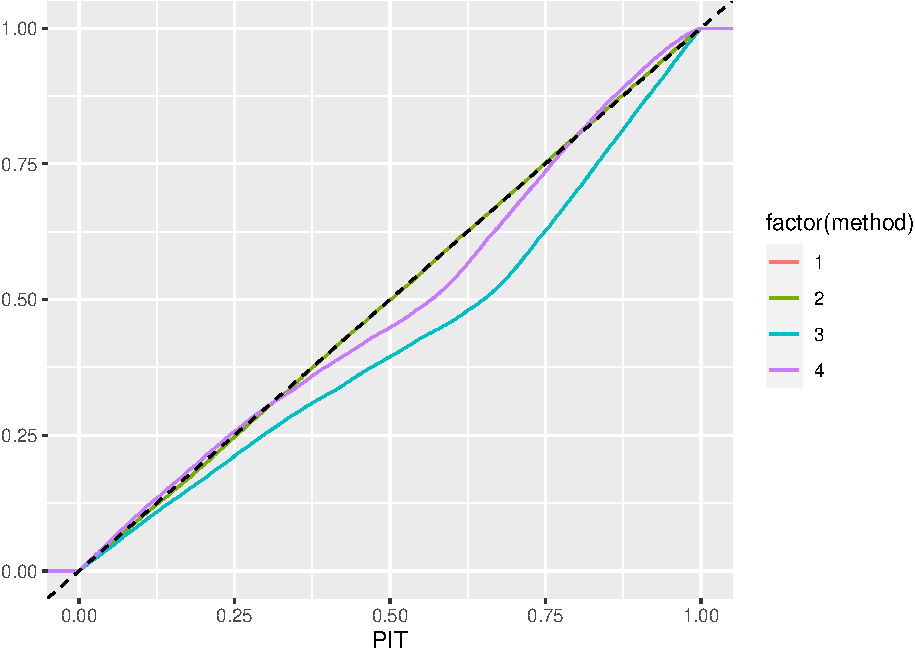
\includegraphics{ensemble_calibration_files/figure-latex/unnamed-chunk-10-1} 

}

\caption{PIT Histograms for Training Seasons}\label{fig:unnamed-chunk-10}
\end{figure}

\newpage

\begin{figure}[H]

{\centering \includegraphics{ensemble_calibration_files/figure-latex/fig1-1} 

}

\caption{PIT Histograms for Test Season 2016/2017}\label{fig:fig1}
\end{figure}

\begin{itemize}
\item There is evidence of bias in the PIT histograms in both the training and test seasons. The BLP, which outperforms other methods, has a more uniform PIT histogram in the test season.
\item The training PIT histograms for BMC2, EW-BLP, and EW-BMC2 look more uniform compared to that of BLP, maybe overfitting?
\end{itemize}

\newpage

\hypertarget{week-ahead-1}{%
\subsubsection{2 Week Ahead}\label{week-ahead-1}}

\begin{figure}[H]

{\centering 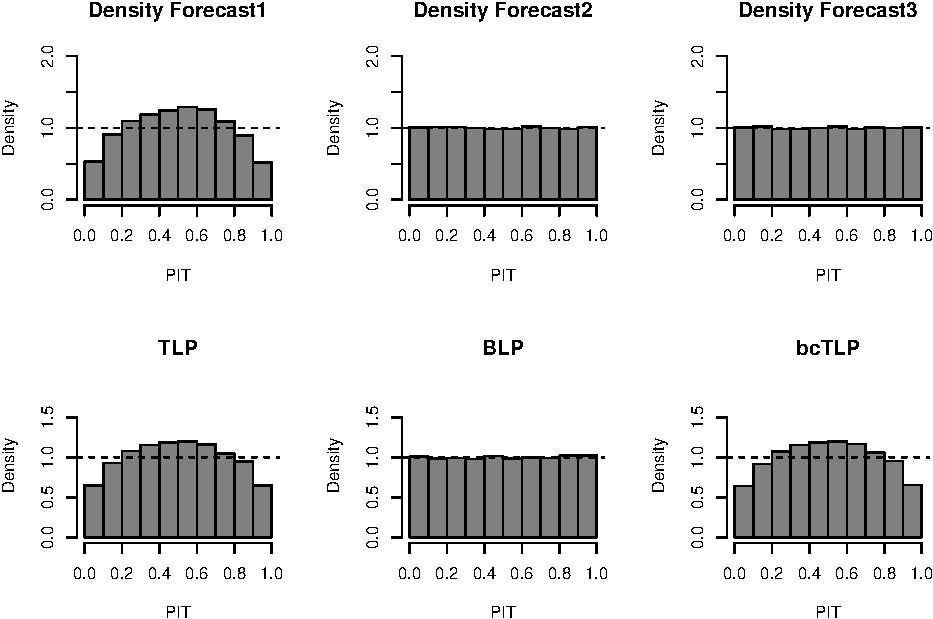
\includegraphics{ensemble_calibration_files/figure-latex/unnamed-chunk-11-1} 

}

\caption{PIT Histograms for Training Seasons}\label{fig:unnamed-chunk-11}
\end{figure}

\newpage

\begin{figure}[H]

{\centering \includegraphics{ensemble_calibration_files/figure-latex/fig2-1} 

}

\caption{PIT Histograms for Test Season 2016/2017}\label{fig:fig2}
\end{figure}

\begin{itemize}
\item There is evidence of some bias in the PIT histograms in both the training and test seasons but less than the previous target. The BLP, which outperforms other methods, has a more uniform PIT histogram in the test season.
\end{itemize}

\newpage

\hypertarget{week-ahead-2}{%
\subsubsection{3 Week Ahead}\label{week-ahead-2}}

\begin{figure}[H]

{\centering 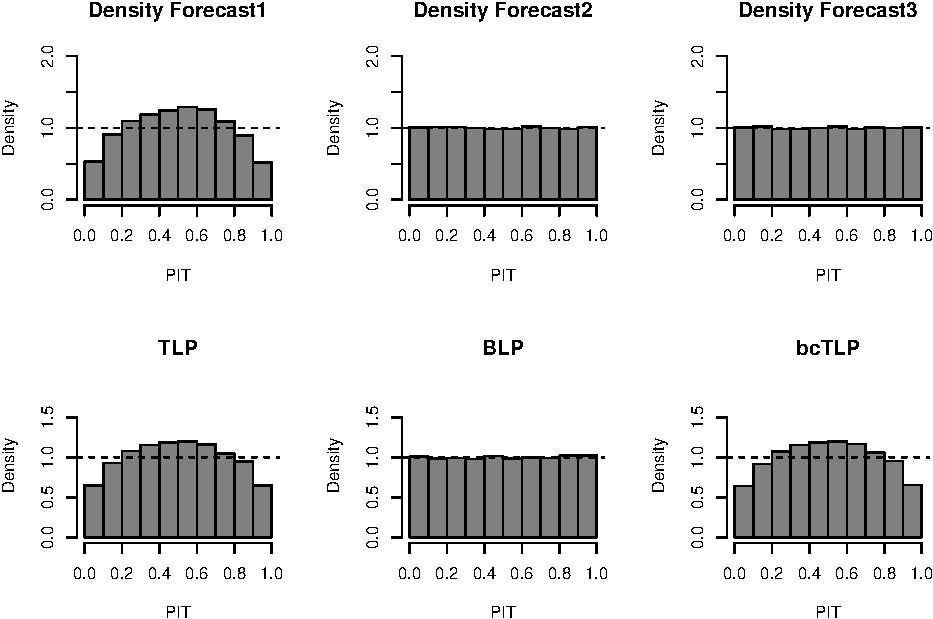
\includegraphics{ensemble_calibration_files/figure-latex/unnamed-chunk-12-1} 

}

\caption{PIT Histograms for Training Seasons}\label{fig:unnamed-chunk-12}
\end{figure}

\newpage

\begin{figure}[H]

{\centering \includegraphics{ensemble_calibration_files/figure-latex/fig3-1} 

}

\caption{PIT Histograms for Test Season 2016/2017}\label{fig:fig3}
\end{figure}

\begin{itemize}
\item There is evidence of some bias in the PIT histograms in both the training and test seasons. The BLP, which outperforms other methods, has a more uniform PIT histogram in the test season.
\item There might be some overfitting going on, the train PIT histograms look a lot better than the test PIT histograms.
\end{itemize}

\newpage

\hypertarget{week-ahead-3}{%
\subsubsection{4 Week Ahead}\label{week-ahead-3}}

\begin{figure}[H]

{\centering 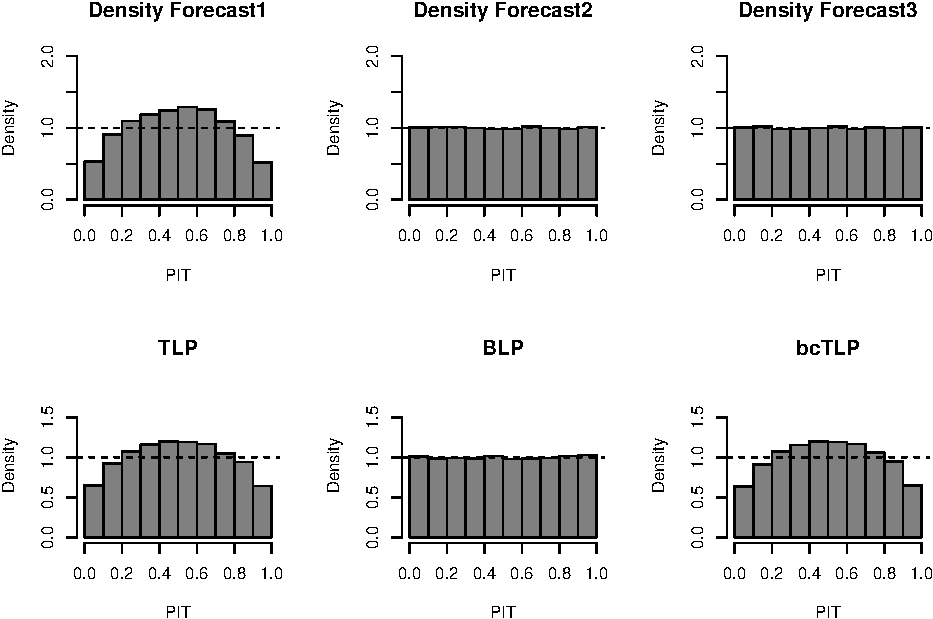
\includegraphics{ensemble_calibration_files/figure-latex/unnamed-chunk-13-1} 

}

\caption{PIT Histograms for Training Seasons}\label{fig:unnamed-chunk-13}
\end{figure}

\newpage

\begin{figure}[H]

{\centering \includegraphics{ensemble_calibration_files/figure-latex/fig4-1} 

}

\caption{PIT Histograms for Test Season 2016/2017}\label{fig:fig4}
\end{figure}

\begin{itemize}
\item There is evidence of a little bias in the PIT histograms in both the training and test seasons. 
\item The BLP, EW-BLP, BMC2, and EW-BMC2 are relatively well-calibrated in the training seasons which outperforms other methods, has a more uniform PIT histogram in the test season.
\item TLP outperforms other methods in terms of mean test log score, but the beta methods seem to have more uniform PIT histograms.
\end{itemize}

\newpage

\hypertarget{test-season-20172018}{%
\subsection{Test season 2017/2018}\label{test-season-20172018}}

\hypertarget{week-ahead-4}{%
\subsubsection{1 Week Ahead}\label{week-ahead-4}}

\begin{figure}[H]

{\centering 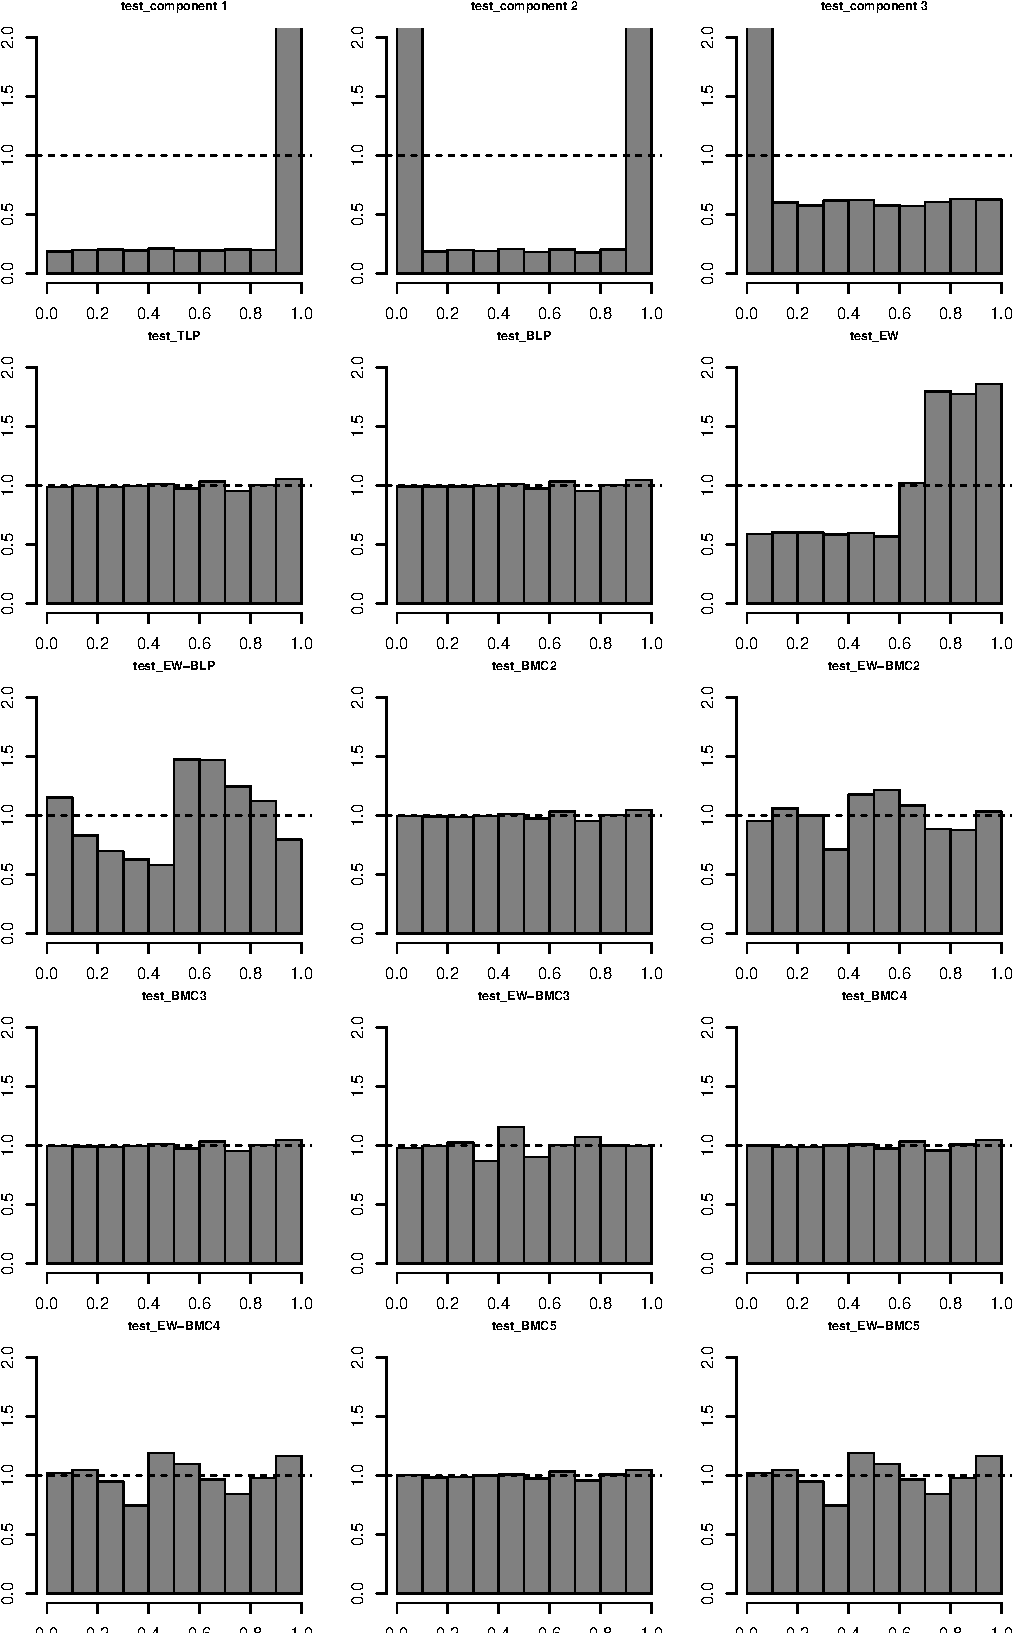
\includegraphics{ensemble_calibration_files/figure-latex/unnamed-chunk-14-1} 

}

\caption{PIT Histograms for Training Seasons}\label{fig:unnamed-chunk-14}
\end{figure}

\newpage

\begin{figure}[H]

{\centering \includegraphics{ensemble_calibration_files/figure-latex/fig5-1} 

}

\caption{PIT Histograms for Test Season 2017/2018}\label{fig:fig5}
\end{figure}

\begin{itemize}
\item There is evidence of some bias in the PIT histograms in both the training and test seasons. The BLP, which outperforms other methods, has a more uniform PIT histogram in the test season, but it is not very calibrated.
\end{itemize}

\newpage

\hypertarget{week-ahead-5}{%
\subsubsection{2 Week Ahead}\label{week-ahead-5}}

\begin{figure}[H]

{\centering 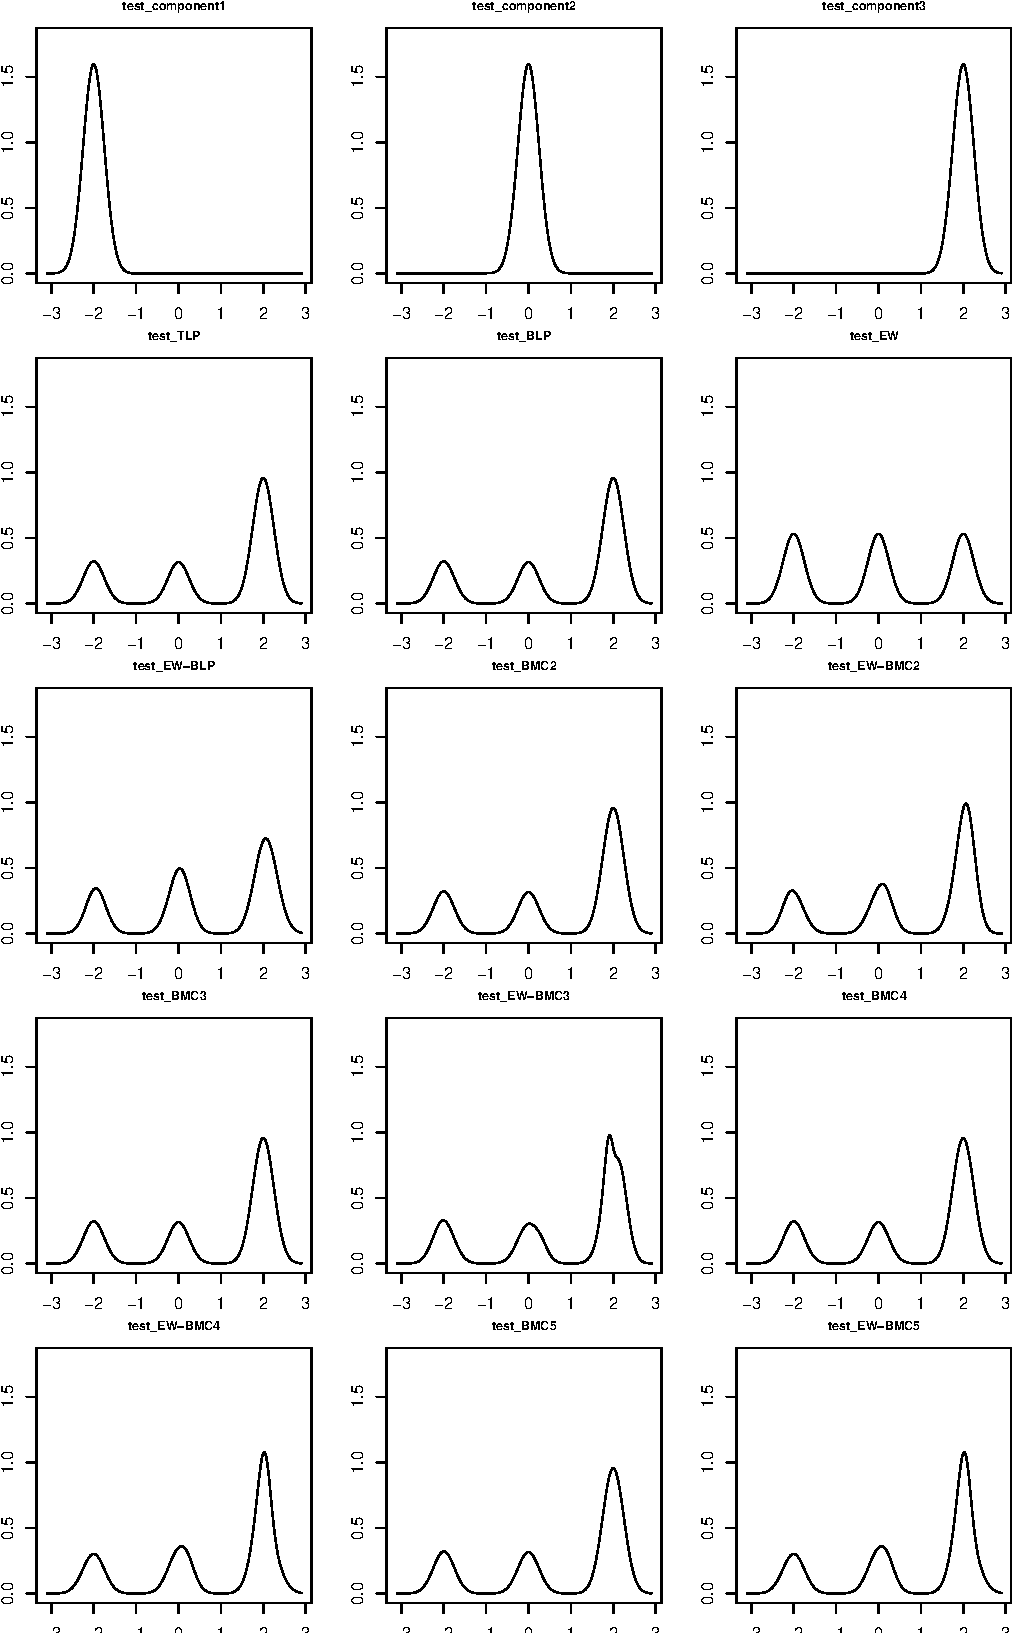
\includegraphics{ensemble_calibration_files/figure-latex/unnamed-chunk-15-1} 

}

\caption{PIT Histograms for Training Seasons}\label{fig:unnamed-chunk-15}
\end{figure}

\newpage

\begin{figure}[H]

{\centering \includegraphics{ensemble_calibration_files/figure-latex/fig6-1} 

}

\caption{PIT Histograms for Test Season 2017/2018}\label{fig:fig6}
\end{figure}

\begin{itemize}
\item There is evidence of some bias in the PIT histograms in both the training and test seasons. Overall the PIT histograms for the beta methods do not look uniform for the test season, despite being relatively well calibrated for the training seasons
\item The BLP, which outperforms other methods, does not seem to be more calibrated than the TLP in the test season.
\end{itemize}

\newpage

\hypertarget{week-ahead-6}{%
\subsubsection{3 Week Ahead}\label{week-ahead-6}}

\begin{figure}[H]

{\centering 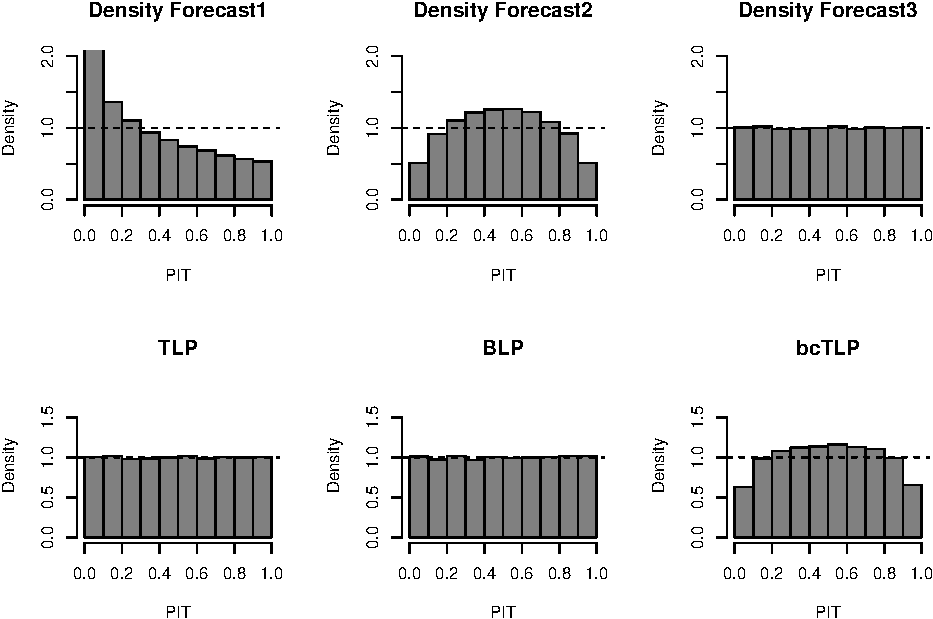
\includegraphics{ensemble_calibration_files/figure-latex/unnamed-chunk-16-1} 

}

\caption{PIT Histograms for Training Seasons}\label{fig:unnamed-chunk-16}
\end{figure}

\newpage

\begin{figure}[H]

{\centering \includegraphics{ensemble_calibration_files/figure-latex/fig7-1} 

}

\caption{PIT Histograms for Test Season 2017/2018}\label{fig:fig7}
\end{figure}

\begin{itemize}
\item We have a similar situation here as in the previous target of the same year, but the tail calibration is much worse.
\item BMC2 is the best performing method in terms of mean log score, but again it does not seem more calibrated than TLP (or worse even).
\end{itemize}

\newpage

\hypertarget{week-ahead-7}{%
\subsubsection{4 Week Ahead}\label{week-ahead-7}}

\begin{figure}[H]

{\centering \includegraphics{ensemble_calibration_files/figure-latex/unnamed-chunk-17-1} 

}

\caption{PIT Histograms for Training Seasons}\label{fig:unnamed-chunk-17}
\end{figure}

\newpage

\begin{figure}[H]

{\centering \includegraphics{ensemble_calibration_files/figure-latex/fig8-1} 

}

\caption{PIT Histograms for Test Season 2017/2018}\label{fig:fig8}
\end{figure}

\begin{itemize}
\item PIT histograms for the training season look well calibrated, but very uncalibrated for the test seasons.
\item TLP outperforms other methods here in terms of log score, and the PIT histograms agree.
\item For this season, it is possible the poor calibration is a result from training seasons being very different from the test season (bad flu season in 2017/2018), so we have a lot of overfitting. This phenomenon is more apparent for 3-4 week ahead targets.
\end{itemize}

\newpage

\hypertarget{test-season-20182019}{%
\subsection{Test season 2018/2019}\label{test-season-20182019}}

\hypertarget{week-ahead-8}{%
\subsubsection{1 Week Ahead}\label{week-ahead-8}}

\begin{figure}[H]

{\centering 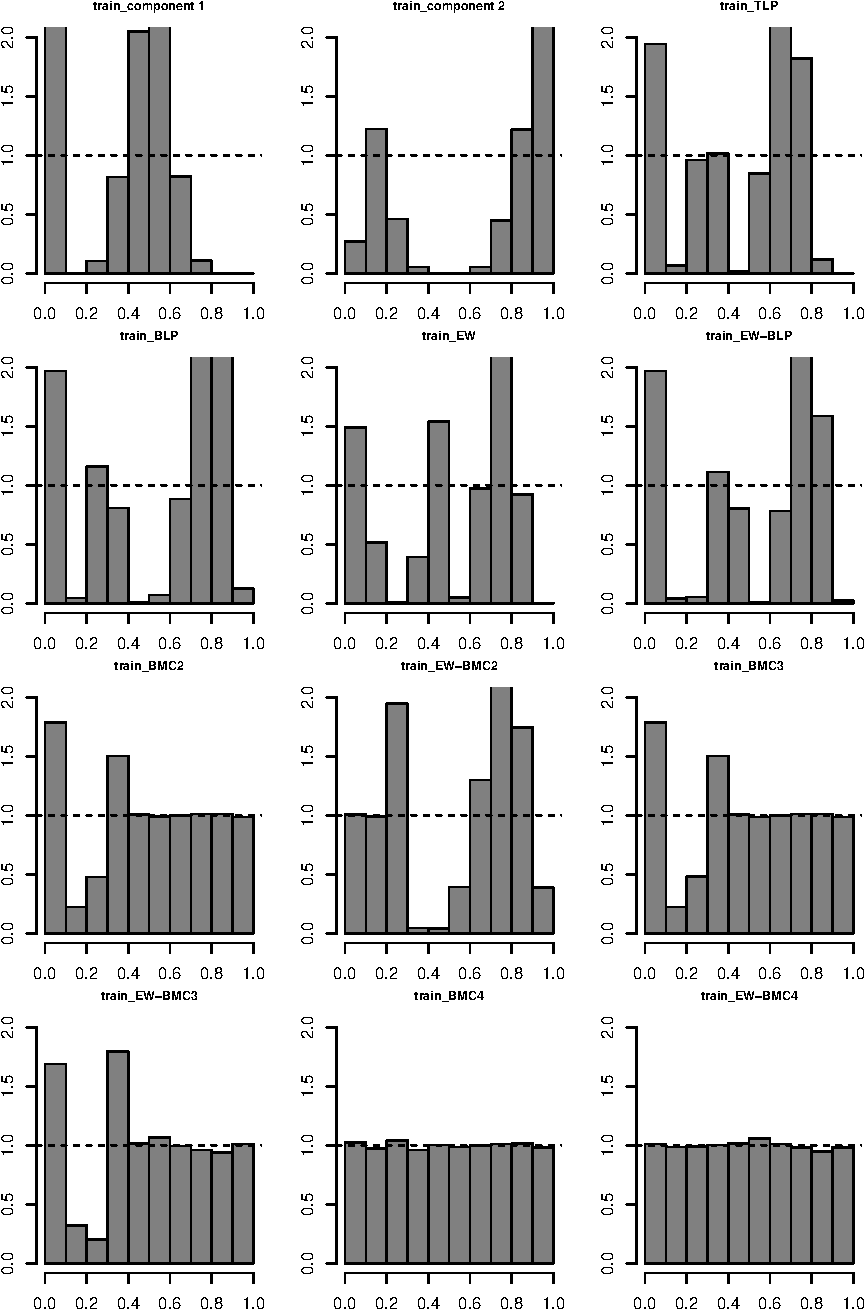
\includegraphics{ensemble_calibration_files/figure-latex/unnamed-chunk-18-1} 

}

\caption{PIT Histograms for Training Seasons}\label{fig:unnamed-chunk-18}
\end{figure}

\newpage

\begin{figure}[H]

{\centering \includegraphics{ensemble_calibration_files/figure-latex/fig9-1} 

}

\caption{PIT Histograms for Test Season 2018/2019}\label{fig:fig9}
\end{figure}

\begin{itemize}
\item There is evidence of some bias in the PIT histograms in the training seasons, but look more calibrated for the test season.
\item The BMC2, which outperforms other methods, does not seem to have a more uniform PIT histogram in the test season compared to other beta methods.
\end{itemize}

\newpage

\hypertarget{week-ahead-9}{%
\subsubsection{2 Week Ahead}\label{week-ahead-9}}

\begin{figure}[H]

{\centering 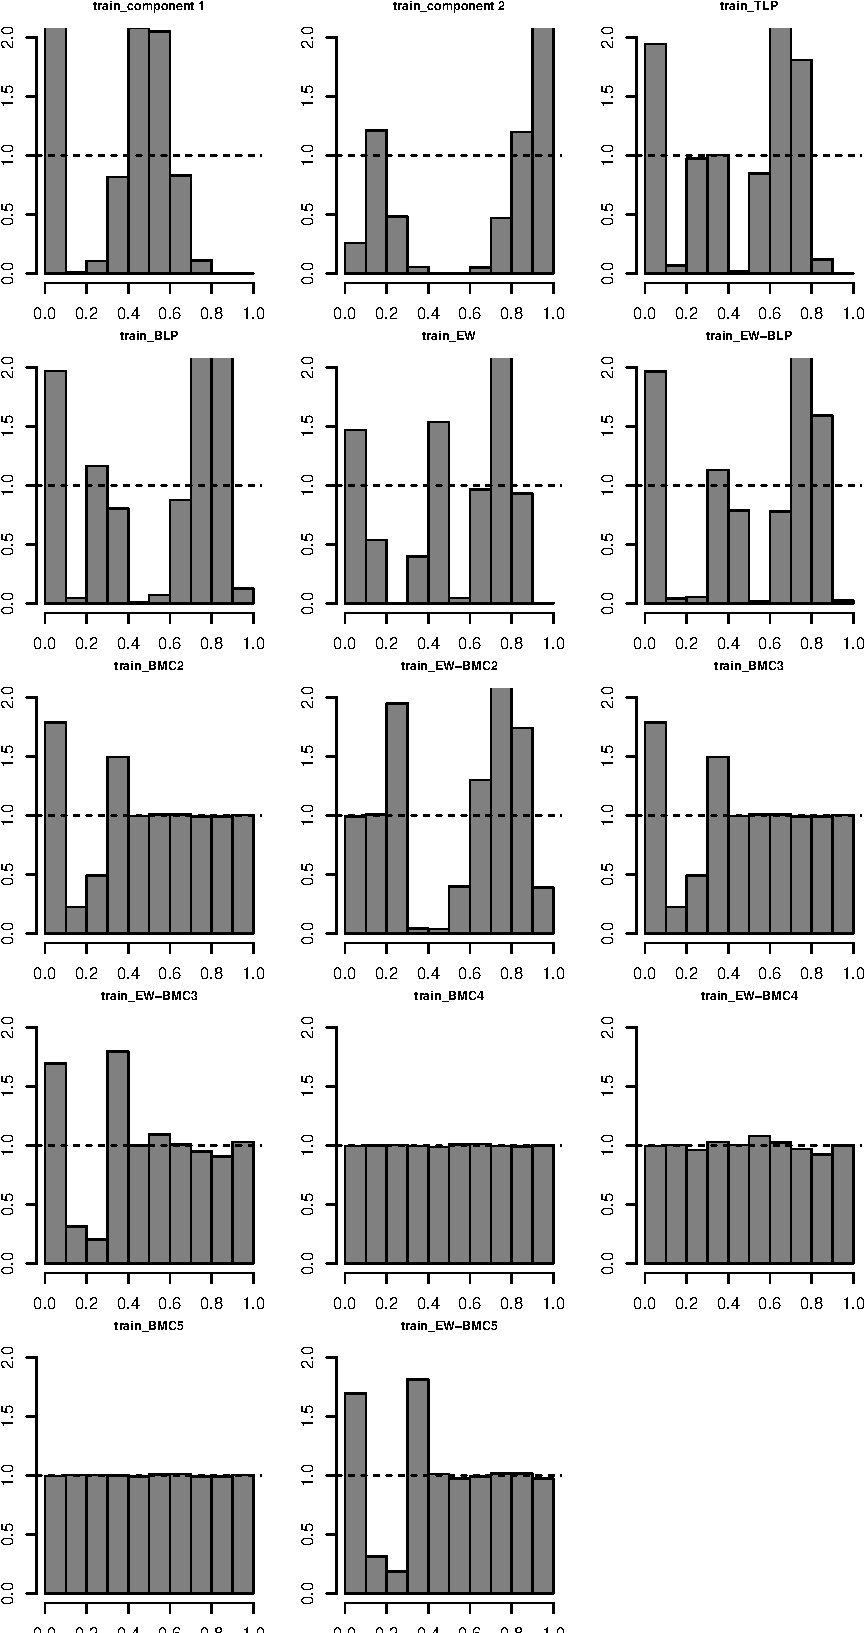
\includegraphics{ensemble_calibration_files/figure-latex/unnamed-chunk-19-1} 

}

\caption{PIT Histograms for Training Seasons}\label{fig:unnamed-chunk-19}
\end{figure}

\newpage

\begin{figure}[H]

{\centering \includegraphics{ensemble_calibration_files/figure-latex/fig10-1} 

}

\caption{PIT Histograms for Test Season 2018/2019}\label{fig:fig10}
\end{figure}

\begin{itemize}
\item The PIT histograms in the training and test seasons look similar for the beta methods. The BLP, which outperforms other methods, has a more uniform PIT histogram in the test season.
\item There is evidence of bias.
\end{itemize}

\newpage

\hypertarget{week-ahead-10}{%
\subsubsection{3 Week Ahead}\label{week-ahead-10}}

\begin{figure}[H]

{\centering 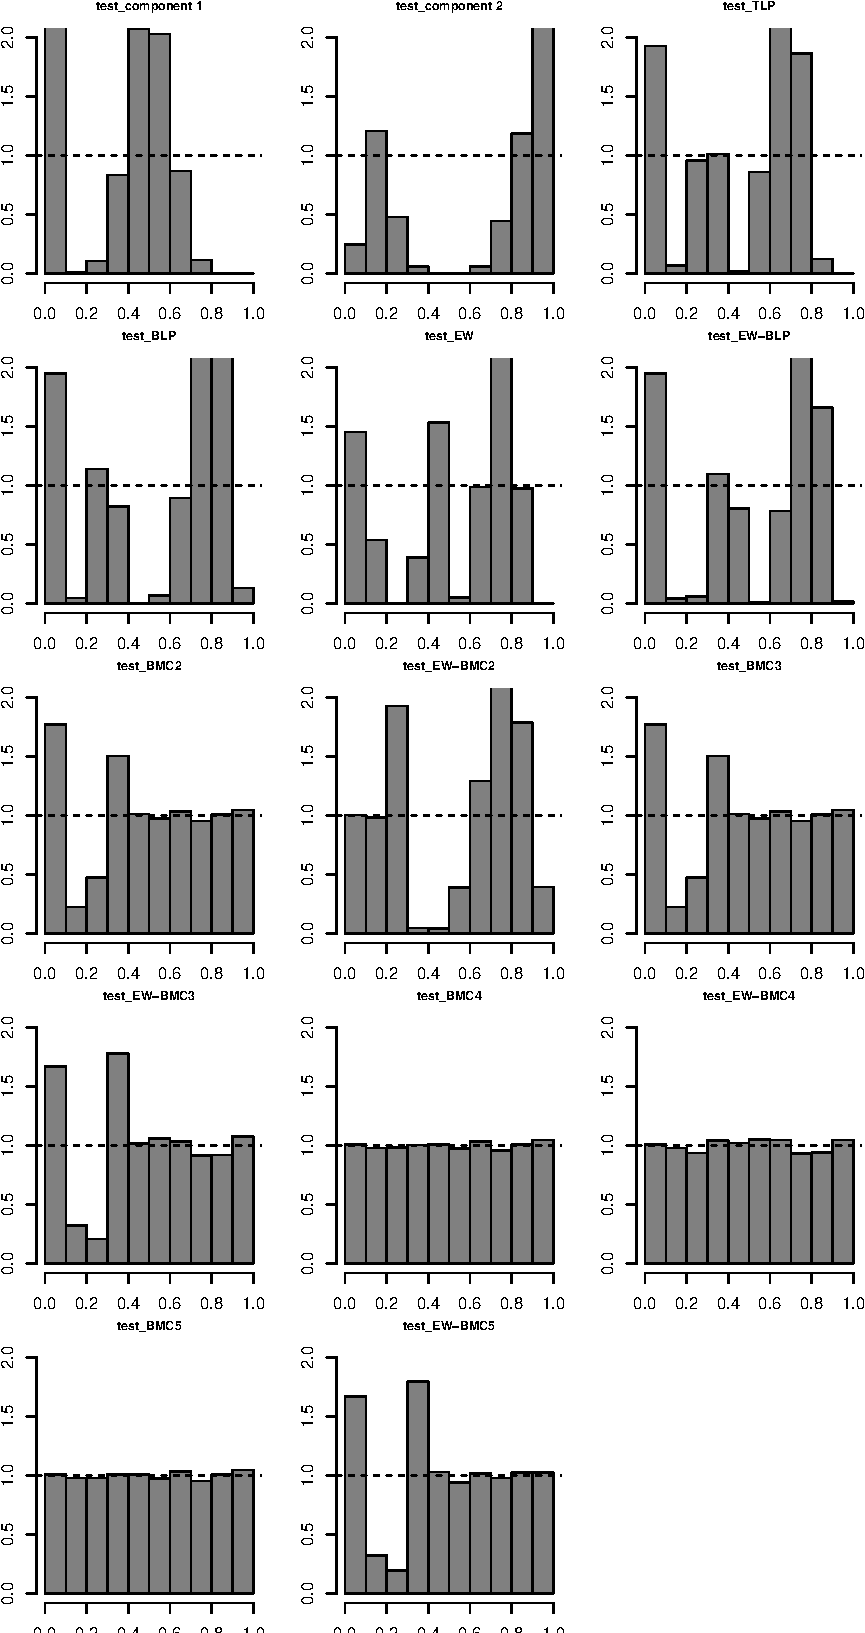
\includegraphics{ensemble_calibration_files/figure-latex/unnamed-chunk-20-1} 

}

\caption{PIT Histograms for Training Seasons}\label{fig:unnamed-chunk-20}
\end{figure}

\newpage

\begin{figure}[H]

{\centering \includegraphics{ensemble_calibration_files/figure-latex/fig11-1} 

}

\caption{PIT Histograms for Test Season 2018/2019}\label{fig:fig11}
\end{figure}

\begin{itemize}
\item There is evidence of some bias in the PIT histograms in the test season, but look more calibrated for the training seasons (no surprise here).
\item The BMC2, which outperforms other methods, does not seem to have a more uniform PIT histogram in the test season compared to other beta methods.
\end{itemize}

\newpage

\hypertarget{week-ahead-11}{%
\subsubsection{4 Week Ahead}\label{week-ahead-11}}

\begin{figure}[H]

{\centering 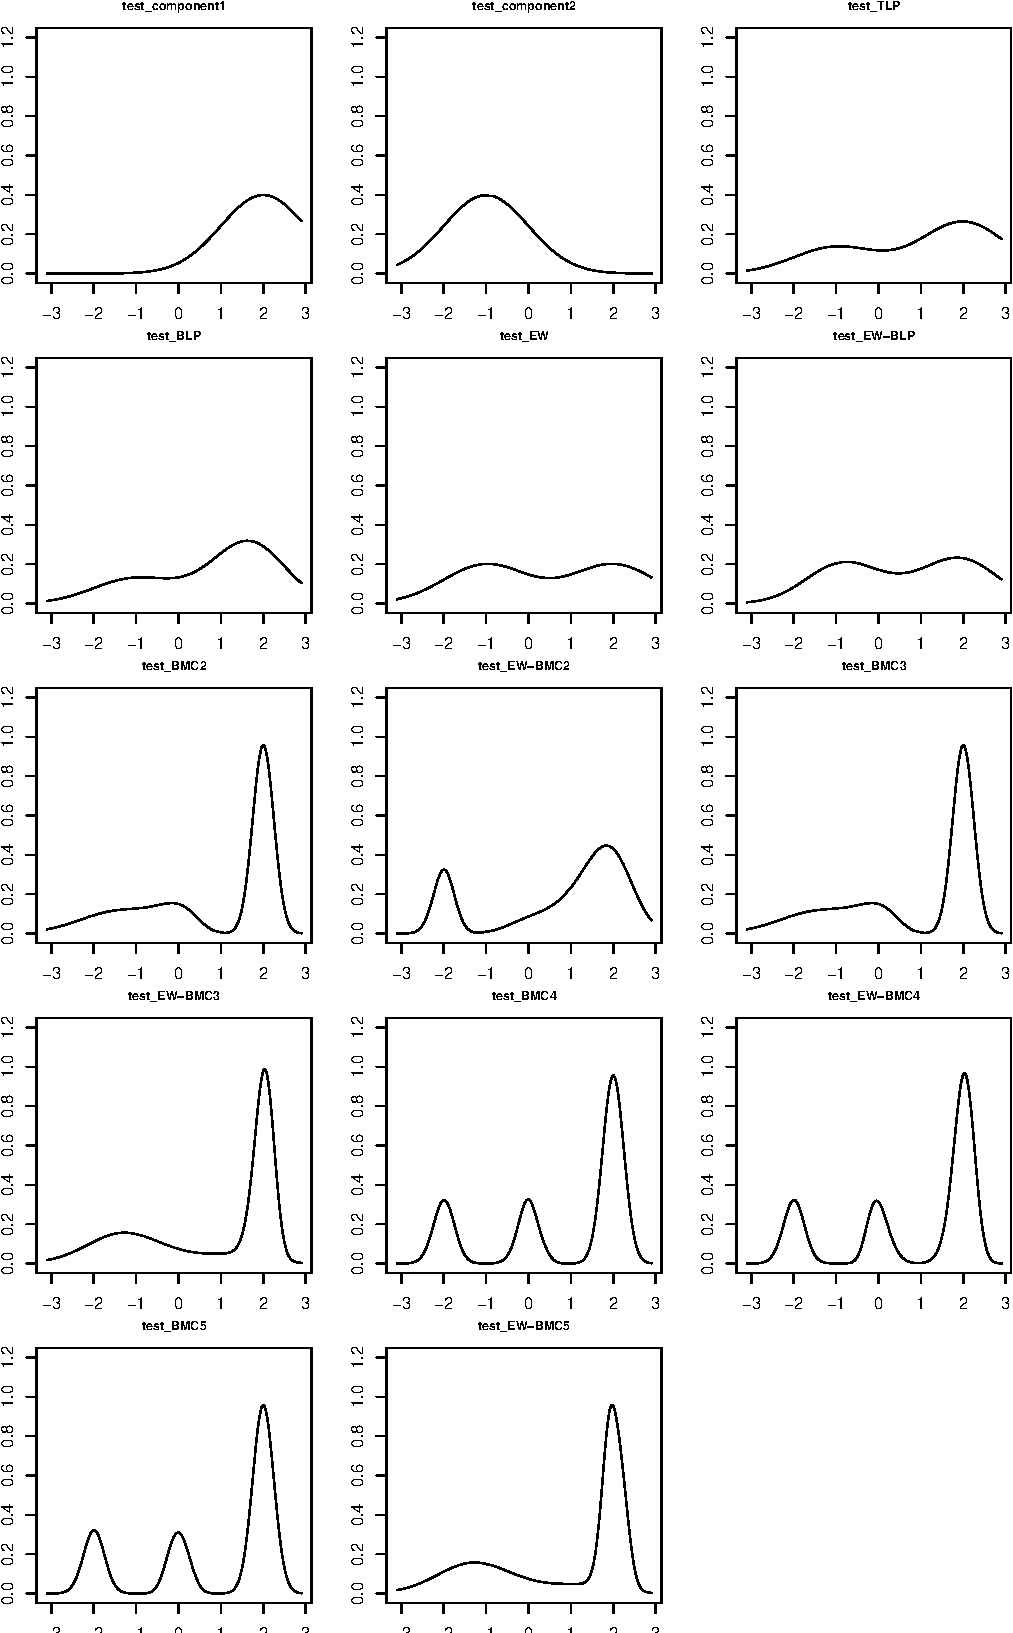
\includegraphics{ensemble_calibration_files/figure-latex/unnamed-chunk-21-1} 

}

\caption{PIT Histograms for Training Seasons}\label{fig:unnamed-chunk-21}
\end{figure}

\newpage

\begin{figure}[H]

{\centering \includegraphics{ensemble_calibration_files/figure-latex/fig12-1} 

}

\caption{PIT Histograms for Test Season 2018/2019}\label{fig:fig12}
\end{figure}

\begin{itemize}
\item We see a lot bias in the PIT histograms in test seasons, especially for the equally-weighted beta methods, despite the PIT histograms looking well-calibrated for the training seasons.
\item The BMC2, which outperforms other methods, has a more uniform PIT histogram in the test season compared to other methods. However, these don't look well-calibrated overall.
\end{itemize}

\hypertarget{estimated-parameters}{%
\section{Estimated Parameters}\label{estimated-parameters}}

\hypertarget{test-season-20162017-1}{%
\subsection{Test season 2016/2017}\label{test-season-20162017-1}}

\hypertarget{week-ahead-12}{%
\subsubsection{1 Week Ahead}\label{week-ahead-12}}

\begin{tabular}{lrrrrrr}
\toprule
Method & $w_1$ & $w_2$ & $\alpha_1$ & $\beta_1$ & $\alpha_2$ & $\beta_2$\\
\midrule
TLP & NA & NA & NA & NA & NA & NA\\
EW & NA & NA & NA & NA & NA & NA\\
BLP & NA & NA & 0.500 & 7.021 & NA & NA\\
EW-BLP & NA & NA & 0.495 & 7.224 & NA & NA\\
BMC2 & 0.508 & 0.492 & 0.611 & 11.028 & 0.383 & 10.797\\
EW-BMC2 & 0.291 & 0.709 & 0.363 & 10.336 & 0.550 & 9.107\\
\bottomrule
\end{tabular}

\begin{tabular}{lrrrrrrrrrrrrr}
\toprule
Method & $\omega_{11}$ & $\omega_{12}$ & $\omega_{13}$ & $\omega_{14}$ & $\omega_{15}$ & $\omega_{16}$ & $\omega_{17}$ & $\omega_{18}$ & $\omega_{19}$ & $\omega_{110}$ & $\omega_{111}$ & $\omega_{112}$ & $\omega_{113}$\\
\midrule
TLP & 0.017 & 0.002 & 0.027 & 0.004 & 0.010 & 0.001 & 0.000 & 0.000 & 0.000 & 0.000 & 0.001 & 0.158 & 0.000\\
EW & 0.037 & 0.037 & 0.037 & 0.037 & 0.037 & 0.037 & 0.037 & 0.037 & 0.037 & 0.037 & 0.037 & 0.037 & 0.037\\
BLP & 0.047 & 0.045 & 0.042 & 0.037 & 0.033 & 0.018 & 0.002 & 0.000 & 0.184 & 0.000 & 0.000 & 0.025 & 0.000\\
EW-BLP & 0.037 & 0.037 & 0.037 & 0.037 & 0.037 & 0.037 & 0.037 & 0.037 & 0.037 & 0.037 & 0.037 & 0.037 & 0.037\\
BMC2 & 0.033 & 0.047 & 0.057 & 0.033 & 0.008 & 0.044 & 0.001 & 0.024 & 0.105 & 0.000 & 0.000 & 0.023 & 0.000\\
EW-BMC2 & 0.037 & 0.037 & 0.037 & 0.037 & 0.037 & 0.037 & 0.037 & 0.037 & 0.037 & 0.037 & 0.037 & 0.037 & 0.037\\
\bottomrule
\end{tabular}

\begin{tabular}{lrrrrrrrrrrrrrr}
\toprule
Method & $\omega_{114}$ & $\omega_{115}$ & $\omega_{116}$ & $\omega_{117}$ & $\omega_{118}$ & $\omega_{119}$ & $\omega_{120}$ & $\omega_{121}$ & $\omega_{122}$ & $\omega_{123}$ & $\omega_{124}$ & $\omega_{125}$ & $\omega_{126}$ & $\omega_{127}$\\
\midrule
TLP & 0.049 & 0.150 & 0.000 & 0.000 & 0.366 & 0.002 & 0.000 & 0.215 & 0.000 & 0.000 & 0.000 & 0.000 & 0.000 & 0.000\\
EW & 0.037 & 0.037 & 0.037 & 0.037 & 0.037 & 0.037 & 0.037 & 0.037 & 0.037 & 0.037 & 0.037 & 0.037 & 0.037 & 0.037\\
BLP & 0.086 & 0.028 & 0.000 & 0.000 & 0.096 & 0.141 & 0.052 & 0.002 & 0.003 & 0.003 & 0.000 & 0.000 & 0.126 & 0.029\\
EW-BLP & 0.037 & 0.037 & 0.037 & 0.037 & 0.037 & 0.037 & 0.037 & 0.037 & 0.037 & 0.037 & 0.037 & 0.037 & 0.037 & 0.037\\
BMC2 & 0.120 & 0.000 & 0.000 & 0.009 & 0.094 & 0.045 & 0.097 & 0.001 & 0.002 & 0.002 & 0.000 & 0.000 & 0.196 & 0.058\\
EW-BMC2 & 0.037 & 0.037 & 0.037 & 0.037 & 0.037 & 0.037 & 0.037 & 0.037 & 0.037 & 0.037 & 0.037 & 0.037 & 0.037 & 0.037\\
\bottomrule
\end{tabular}

\begin{tabular}{lrrrrrrrrrrrrr}
\toprule
Method & $\omega_{21}$ & $\omega_{22}$ & $\omega_{23}$ & $\omega_{24}$ & $\omega_{25}$ & $\omega_{26}$ & $\omega_{27}$ & $\omega_{28}$ & $\omega_{29}$ & $\omega_{210}$ & $\omega_{211}$ & $\omega_{212}$ & $\omega_{213}$\\
\midrule
TLP & NA & NA & NA & NA & NA & NA & NA & NA & NA & NA & NA & NA & NA\\
EW & NA & NA & NA & NA & NA & NA & NA & NA & NA & NA & NA & NA & NA\\
BLP & NA & NA & NA & NA & NA & NA & NA & NA & NA & NA & NA & NA & NA\\
EW-BLP & NA & NA & NA & NA & NA & NA & NA & NA & NA & NA & NA & NA & NA\\
BMC2 & 0.033 & 0.044 & 0.055 & 0.032 & 0.008 & 0.041 & 0.008 & 0.000 & 0.215 & 0.058 & 0.000 & 0.015 & 0.010\\
EW-BMC2 & 0.037 & 0.037 & 0.037 & 0.037 & 0.037 & 0.037 & 0.037 & 0.037 & 0.037 & 0.037 & 0.037 & 0.037 & 0.037\\
\bottomrule
\end{tabular}

\begin{tabular}{lrrrrrrrrrrrrrr}
\toprule
Method & $\omega_{214}$ & $\omega_{215}$ & $\omega_{216}$ & $\omega_{217}$ & $\omega_{218}$ & $\omega_{219}$ & $\omega_{220}$ & $\omega_{221}$ & $\omega_{222}$ & $\omega_{223}$ & $\omega_{224}$ & $\omega_{225}$ & $\omega_{226}$ & $\omega_{227}$\\
\midrule
TLP & NA & NA & NA & NA & NA & NA & NA & NA & NA & NA & NA & NA & NA & NA\\
EW & NA & NA & NA & NA & NA & NA & NA & NA & NA & NA & NA & NA & NA & NA\\
BLP & NA & NA & NA & NA & NA & NA & NA & NA & NA & NA & NA & NA & NA & NA\\
EW-BLP & NA & NA & NA & NA & NA & NA & NA & NA & NA & NA & NA & NA & NA & NA\\
BMC2 & 0.000 & 0.113 & 0.000 & 0.000 & 0.083 & 0.207 & 0.000 & 0.001 & 0.000 & 0.000 & 0.004 & 0.000 & 0.072 & 0.000\\
EW-BMC2 & 0.037 & 0.037 & 0.037 & 0.037 & 0.037 & 0.037 & 0.037 & 0.037 & 0.037 & 0.037 & 0.037 & 0.037 & 0.037 & 0.037\\
\bottomrule
\end{tabular}

\hypertarget{week-ahead-13}{%
\subsubsection{2 Week Ahead}\label{week-ahead-13}}

\begin{tabular}{lrrrrrr}
\toprule
Method & $w_1$ & $w_2$ & $\alpha_1$ & $\beta_1$ & $\alpha_2$ & $\beta_2$\\
\midrule
TLP & NA & NA & NA & NA & NA & NA\\
EW & NA & NA & NA & NA & NA & NA\\
BLP & NA & NA & 0.481 & 5.462 & NA & NA\\
EW-BLP & NA & NA & 0.458 & 6.166 & NA & NA\\
BMC2 & 0.501 & 0.499 & 0.339 & 8.534 & 0.607 & 8.411\\
EW-BMC2 & 0.888 & 0.112 & 0.423 & 7.747 & 0.720 & 15.005\\
\bottomrule
\end{tabular}

\begin{tabular}{lrrrrrrrrrrrrr}
\toprule
Method & $\omega_{11}$ & $\omega_{12}$ & $\omega_{13}$ & $\omega_{14}$ & $\omega_{15}$ & $\omega_{16}$ & $\omega_{17}$ & $\omega_{18}$ & $\omega_{19}$ & $\omega_{110}$ & $\omega_{111}$ & $\omega_{112}$ & $\omega_{113}$\\
\midrule
TLP & 0.091 & 0.000 & 0.144 & 0.000 & 0.043 & 0.000 & 0.000 & 0.000 & 0.000 & 0.000 & 0.206 & 0.056 & 0.000\\
EW & 0.037 & 0.037 & 0.037 & 0.037 & 0.037 & 0.037 & 0.037 & 0.037 & 0.037 & 0.037 & 0.037 & 0.037 & 0.037\\
BLP & 0.006 & 0.001 & 0.023 & 0.014 & 0.000 & 0.189 & 0.008 & 0.000 & 0.001 & 0.036 & 0.126 & 0.000 & 0.000\\
EW-BLP & 0.037 & 0.037 & 0.037 & 0.037 & 0.037 & 0.037 & 0.037 & 0.037 & 0.037 & 0.037 & 0.037 & 0.037 & 0.037\\
BMC2 & 0.012 & 0.000 & 0.073 & 0.000 & 0.000 & 0.249 & 0.028 & 0.000 & 0.000 & 0.000 & 0.150 & 0.000 & 0.000\\
EW-BMC2 & 0.037 & 0.037 & 0.037 & 0.037 & 0.037 & 0.037 & 0.037 & 0.037 & 0.037 & 0.037 & 0.037 & 0.037 & 0.037\\
\bottomrule
\end{tabular}

\begin{tabular}{lrrrrrrrrrrrrrr}
\toprule
Method & $\omega_{114}$ & $\omega_{115}$ & $\omega_{116}$ & $\omega_{117}$ & $\omega_{118}$ & $\omega_{119}$ & $\omega_{120}$ & $\omega_{121}$ & $\omega_{122}$ & $\omega_{123}$ & $\omega_{124}$ & $\omega_{125}$ & $\omega_{126}$ & $\omega_{127}$\\
\midrule
TLP & 0.000 & 0.197 & 0.000 & 0.000 & 0.113 & 0.000 & 0.000 & 0.149 & 0.000 & 0.000 & 0.000 & 0.000 & 0.000 & 0.000\\
EW & 0.037 & 0.037 & 0.037 & 0.037 & 0.037 & 0.037 & 0.037 & 0.037 & 0.037 & 0.037 & 0.037 & 0.037 & 0.037 & 0.037\\
BLP & 0.024 & 0.101 & 0.000 & 0.009 & 0.120 & 0.133 & 0.025 & 0.000 & 0.001 & 0.001 & 0.000 & 0.000 & 0.138 & 0.042\\
EW-BLP & 0.037 & 0.037 & 0.037 & 0.037 & 0.037 & 0.037 & 0.037 & 0.037 & 0.037 & 0.037 & 0.037 & 0.037 & 0.037 & 0.037\\
BMC2 & 0.012 & 0.106 & 0.000 & 0.000 & 0.052 & 0.199 & 0.000 & 0.000 & 0.002 & 0.022 & 0.000 & 0.000 & 0.095 & 0.000\\
EW-BMC2 & 0.037 & 0.037 & 0.037 & 0.037 & 0.037 & 0.037 & 0.037 & 0.037 & 0.037 & 0.037 & 0.037 & 0.037 & 0.037 & 0.037\\
\bottomrule
\end{tabular}

\begin{tabular}{lrrrrrrrrrrrrr}
\toprule
Method & $\omega_{21}$ & $\omega_{22}$ & $\omega_{23}$ & $\omega_{24}$ & $\omega_{25}$ & $\omega_{26}$ & $\omega_{27}$ & $\omega_{28}$ & $\omega_{29}$ & $\omega_{210}$ & $\omega_{211}$ & $\omega_{212}$ & $\omega_{213}$\\
\midrule
TLP & NA & NA & NA & NA & NA & NA & NA & NA & NA & NA & NA & NA & NA\\
EW & NA & NA & NA & NA & NA & NA & NA & NA & NA & NA & NA & NA & NA\\
BLP & NA & NA & NA & NA & NA & NA & NA & NA & NA & NA & NA & NA & NA\\
EW-BLP & NA & NA & NA & NA & NA & NA & NA & NA & NA & NA & NA & NA & NA\\
BMC2 & 0.000 & 0.000 & 0.035 & 0.027 & 0.000 & 0.125 & 0.000 & 0.000 & 0.000 & 0.000 & 0.083 & 0.000 & 0.000\\
EW-BMC2 & 0.037 & 0.037 & 0.037 & 0.037 & 0.037 & 0.037 & 0.037 & 0.037 & 0.037 & 0.037 & 0.037 & 0.037 & 0.037\\
\bottomrule
\end{tabular}

\begin{tabular}{lrrrrrrrrrrrrrr}
\toprule
Method & $\omega_{214}$ & $\omega_{215}$ & $\omega_{216}$ & $\omega_{217}$ & $\omega_{218}$ & $\omega_{219}$ & $\omega_{220}$ & $\omega_{221}$ & $\omega_{222}$ & $\omega_{223}$ & $\omega_{224}$ & $\omega_{225}$ & $\omega_{226}$ & $\omega_{227}$\\
\midrule
TLP & NA & NA & NA & NA & NA & NA & NA & NA & NA & NA & NA & NA & NA & NA\\
EW & NA & NA & NA & NA & NA & NA & NA & NA & NA & NA & NA & NA & NA & NA\\
BLP & NA & NA & NA & NA & NA & NA & NA & NA & NA & NA & NA & NA & NA & NA\\
EW-BLP & NA & NA & NA & NA & NA & NA & NA & NA & NA & NA & NA & NA & NA & NA\\
BMC2 & 0.037 & 0.084 & 0.000 & 0.023 & 0.182 & 0.000 & 0.132 & 0.000 & 0.000 & 0.000 & 0.000 & 0.000 & 0.209 & 0.062\\
EW-BMC2 & 0.037 & 0.037 & 0.037 & 0.037 & 0.037 & 0.037 & 0.037 & 0.037 & 0.037 & 0.037 & 0.037 & 0.037 & 0.037 & 0.037\\
\bottomrule
\end{tabular}

\hypertarget{week-ahead-14}{%
\subsubsection{3 Week Ahead}\label{week-ahead-14}}

\begin{tabular}{lrrrrrr}
\toprule
Method & $w_1$ & $w_2$ & $\alpha_1$ & $\beta_1$ & $\alpha_2$ & $\beta_2$\\
\midrule
TLP & NA & NA & NA & NA & NA & NA\\
EW & NA & NA & NA & NA & NA & NA\\
BLP & NA & NA & 0.466 & 5.393 & NA & NA\\
EW-BLP & NA & NA & 0.454 & 6.140 & NA & NA\\
BMC2 & 0.100 & 0.900 & 0.116 & 51.829 & 0.486 & 5.632\\
EW-BMC2 & 0.946 & 0.054 & 0.459 & 5.936 & 0.348 & 64.473\\
\bottomrule
\end{tabular}

\begin{tabular}{lrrrrrrrrrrrrr}
\toprule
Method & $\omega_{11}$ & $\omega_{12}$ & $\omega_{13}$ & $\omega_{14}$ & $\omega_{15}$ & $\omega_{16}$ & $\omega_{17}$ & $\omega_{18}$ & $\omega_{19}$ & $\omega_{110}$ & $\omega_{111}$ & $\omega_{112}$ & $\omega_{113}$\\
\midrule
TLP & 0.115 & 0.000 & 0.093 & 0.000 & 0.041 & 0.000 & 0.000 & 0.008 & 0.000 & 0.000 & 0.183 & 0.041 & 0.000\\
EW & 0.037 & 0.037 & 0.037 & 0.037 & 0.037 & 0.037 & 0.037 & 0.037 & 0.037 & 0.037 & 0.037 & 0.037 & 0.037\\
BLP & 0.001 & 0.035 & 0.061 & 0.023 & 0.007 & 0.118 & 0.027 & 0.000 & 0.002 & 0.045 & 0.145 & 0.000 & 0.000\\
EW-BLP & 0.037 & 0.037 & 0.037 & 0.037 & 0.037 & 0.037 & 0.037 & 0.037 & 0.037 & 0.037 & 0.037 & 0.037 & 0.037\\
BMC2 & 0.002 & 0.130 & 0.719 & 0.000 & 0.003 & 0.002 & 0.035 & 0.000 & 0.000 & 0.000 & 0.011 & 0.050 & 0.000\\
EW-BMC2 & 0.037 & 0.037 & 0.037 & 0.037 & 0.037 & 0.037 & 0.037 & 0.037 & 0.037 & 0.037 & 0.037 & 0.037 & 0.037\\
\bottomrule
\end{tabular}

\begin{tabular}{lrrrrrrrrrrrrrr}
\toprule
Method & $\omega_{114}$ & $\omega_{115}$ & $\omega_{116}$ & $\omega_{117}$ & $\omega_{118}$ & $\omega_{119}$ & $\omega_{120}$ & $\omega_{121}$ & $\omega_{122}$ & $\omega_{123}$ & $\omega_{124}$ & $\omega_{125}$ & $\omega_{126}$ & $\omega_{127}$\\
\midrule
TLP & 0.000 & 0.179 & 0.000 & 0.000 & 0.124 & 0.000 & 0.000 & 0.216 & 0.000 & 0.000 & 0.000 & 0.000 & 0.000 & 0.000\\
EW & 0.037 & 0.037 & 0.037 & 0.037 & 0.037 & 0.037 & 0.037 & 0.037 & 0.037 & 0.037 & 0.037 & 0.037 & 0.037 & 0.037\\
BLP & 0.032 & 0.086 & 0.000 & 0.015 & 0.072 & 0.134 & 0.001 & 0.000 & 0.005 & 0.020 & 0.005 & 0.000 & 0.130 & 0.035\\
EW-BLP & 0.037 & 0.037 & 0.037 & 0.037 & 0.037 & 0.037 & 0.037 & 0.037 & 0.037 & 0.037 & 0.037 & 0.037 & 0.037 & 0.037\\
BMC2 & 0.000 & 0.000 & 0.000 & 0.000 & 0.008 & 0.039 & 0.000 & 0.002 & 0.000 & 0.000 & 0.000 & 0.000 & 0.000 & 0.000\\
EW-BMC2 & 0.037 & 0.037 & 0.037 & 0.037 & 0.037 & 0.037 & 0.037 & 0.037 & 0.037 & 0.037 & 0.037 & 0.037 & 0.037 & 0.037\\
\bottomrule
\end{tabular}

\begin{tabular}{lrrrrrrrrrrrrr}
\toprule
Method & $\omega_{21}$ & $\omega_{22}$ & $\omega_{23}$ & $\omega_{24}$ & $\omega_{25}$ & $\omega_{26}$ & $\omega_{27}$ & $\omega_{28}$ & $\omega_{29}$ & $\omega_{210}$ & $\omega_{211}$ & $\omega_{212}$ & $\omega_{213}$\\
\midrule
TLP & NA & NA & NA & NA & NA & NA & NA & NA & NA & NA & NA & NA & NA\\
EW & NA & NA & NA & NA & NA & NA & NA & NA & NA & NA & NA & NA & NA\\
BLP & NA & NA & NA & NA & NA & NA & NA & NA & NA & NA & NA & NA & NA\\
EW-BLP & NA & NA & NA & NA & NA & NA & NA & NA & NA & NA & NA & NA & NA\\
BMC2 & 0.008 & 0.014 & 0.096 & 0.001 & 0.015 & 0.089 & 0.025 & 0.000 & 0.000 & 0.045 & 0.140 & 0.000 & 0.000\\
EW-BMC2 & 0.037 & 0.037 & 0.037 & 0.037 & 0.037 & 0.037 & 0.037 & 0.037 & 0.037 & 0.037 & 0.037 & 0.037 & 0.037\\
\bottomrule
\end{tabular}

\begin{tabular}{lrrrrrrrrrrrrrr}
\toprule
Method & $\omega_{214}$ & $\omega_{215}$ & $\omega_{216}$ & $\omega_{217}$ & $\omega_{218}$ & $\omega_{219}$ & $\omega_{220}$ & $\omega_{221}$ & $\omega_{222}$ & $\omega_{223}$ & $\omega_{224}$ & $\omega_{225}$ & $\omega_{226}$ & $\omega_{227}$\\
\midrule
TLP & NA & NA & NA & NA & NA & NA & NA & NA & NA & NA & NA & NA & NA & NA\\
EW & NA & NA & NA & NA & NA & NA & NA & NA & NA & NA & NA & NA & NA & NA\\
BLP & NA & NA & NA & NA & NA & NA & NA & NA & NA & NA & NA & NA & NA & NA\\
EW-BLP & NA & NA & NA & NA & NA & NA & NA & NA & NA & NA & NA & NA & NA & NA\\
BMC2 & 0.032 & 0.091 & 0.000 & 0.013 & 0.062 & 0.128 & 0.001 & 0.000 & 0.002 & 0.011 & 0.037 & 0.000 & 0.148 & 0.041\\
EW-BMC2 & 0.037 & 0.037 & 0.037 & 0.037 & 0.037 & 0.037 & 0.037 & 0.037 & 0.037 & 0.037 & 0.037 & 0.037 & 0.037 & 0.037\\
\bottomrule
\end{tabular}

\hypertarget{week-ahead-15}{%
\subsubsection{4 Week Ahead}\label{week-ahead-15}}

\begin{tabular}{lrrrrrr}
\toprule
Method & $w_1$ & $w_2$ & $\alpha_1$ & $\beta_1$ & $\alpha_2$ & $\beta_2$\\
\midrule
TLP & NA & NA & NA & NA & NA & NA\\
EW & NA & NA & NA & NA & NA & NA\\
BLP & NA & NA & 0.465 & 5.675 & NA & NA\\
EW-BLP & NA & NA & 0.452 & 6.001 & NA & NA\\
BMC2 & 0.579 & 0.421 & 0.577 & 9.395 & 0.274 & 11.114\\
EW-BMC2 & 0.615 & 0.385 & 0.453 & 6.000 & 0.451 & 6.004\\
\bottomrule
\end{tabular}

\begin{tabular}{lrrrrrrrrrrrrr}
\toprule
Method & $\omega_{11}$ & $\omega_{12}$ & $\omega_{13}$ & $\omega_{14}$ & $\omega_{15}$ & $\omega_{16}$ & $\omega_{17}$ & $\omega_{18}$ & $\omega_{19}$ & $\omega_{110}$ & $\omega_{111}$ & $\omega_{112}$ & $\omega_{113}$\\
\midrule
TLP & 0.095 & 0.000 & 0.018 & 0.000 & 0.100 & 0.000 & 0.006 & 0.032 & 0.000 & 0.000 & 0.177 & 0.029 & 0.000\\
EW & 0.037 & 0.037 & 0.037 & 0.037 & 0.037 & 0.037 & 0.037 & 0.037 & 0.037 & 0.037 & 0.037 & 0.037 & 0.037\\
BLP & 0.001 & 0.037 & 0.001 & 0.000 & 0.064 & 0.135 & 0.020 & 0.000 & 0.001 & 0.036 & 0.118 & 0.018 & 0.000\\
EW-BLP & 0.037 & 0.037 & 0.037 & 0.037 & 0.037 & 0.037 & 0.037 & 0.037 & 0.037 & 0.037 & 0.037 & 0.037 & 0.037\\
BMC2 & 0.000 & 0.001 & 0.002 & 0.000 & 0.047 & 0.138 & 0.016 & 0.000 & 0.001 & 0.032 & 0.084 & 0.000 & 0.000\\
EW-BMC2 & 0.037 & 0.037 & 0.037 & 0.037 & 0.037 & 0.037 & 0.037 & 0.037 & 0.037 & 0.037 & 0.037 & 0.037 & 0.037\\
\bottomrule
\end{tabular}

\begin{tabular}{lrrrrrrrrrrrrrr}
\toprule
Method & $\omega_{114}$ & $\omega_{115}$ & $\omega_{116}$ & $\omega_{117}$ & $\omega_{118}$ & $\omega_{119}$ & $\omega_{120}$ & $\omega_{121}$ & $\omega_{122}$ & $\omega_{123}$ & $\omega_{124}$ & $\omega_{125}$ & $\omega_{126}$ & $\omega_{127}$\\
\midrule
TLP & 0.034 & 0.113 & 0.000 & 0.000 & 0.112 & 0.000 & 0.000 & 0.284 & 0.000 & 0.000 & 0.000 & 0.000 & 0.000 & 0.000\\
EW & 0.037 & 0.037 & 0.037 & 0.037 & 0.037 & 0.037 & 0.037 & 0.037 & 0.037 & 0.037 & 0.037 & 0.037 & 0.037 & 0.037\\
BLP & 0.054 & 0.049 & 0.000 & 0.027 & 0.000 & 0.157 & 0.000 & 0.001 & 0.016 & 0.012 & 0.060 & 0.013 & 0.142 & 0.038\\
EW-BLP & 0.037 & 0.037 & 0.037 & 0.037 & 0.037 & 0.037 & 0.037 & 0.037 & 0.037 & 0.037 & 0.037 & 0.037 & 0.037 & 0.037\\
BMC2 & 0.015 & 0.084 & 0.000 & 0.049 & 0.022 & 0.063 & 0.000 & 0.000 & 0.000 & 0.000 & 0.210 & 0.000 & 0.186 & 0.049\\
EW-BMC2 & 0.037 & 0.037 & 0.037 & 0.037 & 0.037 & 0.037 & 0.037 & 0.037 & 0.037 & 0.037 & 0.037 & 0.037 & 0.037 & 0.037\\
\bottomrule
\end{tabular}

\begin{tabular}{lrrrrrrrrrrrrr}
\toprule
Method & $\omega_{21}$ & $\omega_{22}$ & $\omega_{23}$ & $\omega_{24}$ & $\omega_{25}$ & $\omega_{26}$ & $\omega_{27}$ & $\omega_{28}$ & $\omega_{29}$ & $\omega_{210}$ & $\omega_{211}$ & $\omega_{212}$ & $\omega_{213}$\\
\midrule
TLP & NA & NA & NA & NA & NA & NA & NA & NA & NA & NA & NA & NA & NA\\
EW & NA & NA & NA & NA & NA & NA & NA & NA & NA & NA & NA & NA & NA\\
BLP & NA & NA & NA & NA & NA & NA & NA & NA & NA & NA & NA & NA & NA\\
EW-BLP & NA & NA & NA & NA & NA & NA & NA & NA & NA & NA & NA & NA & NA\\
BMC2 & 0.080 & 0.036 & 0.154 & 0.000 & 0.140 & 0.000 & 0.029 & 0.000 & 0.000 & 0.000 & 0.126 & 0.043 & 0.000\\
EW-BMC2 & 0.037 & 0.037 & 0.037 & 0.037 & 0.037 & 0.037 & 0.037 & 0.037 & 0.037 & 0.037 & 0.037 & 0.037 & 0.037\\
\bottomrule
\end{tabular}

\begin{tabular}{lrrrrrrrrrrrrrr}
\toprule
Method & $\omega_{214}$ & $\omega_{215}$ & $\omega_{216}$ & $\omega_{217}$ & $\omega_{218}$ & $\omega_{219}$ & $\omega_{220}$ & $\omega_{221}$ & $\omega_{222}$ & $\omega_{223}$ & $\omega_{224}$ & $\omega_{225}$ & $\omega_{226}$ & $\omega_{227}$\\
\midrule
TLP & NA & NA & NA & NA & NA & NA & NA & NA & NA & NA & NA & NA & NA & NA\\
EW & NA & NA & NA & NA & NA & NA & NA & NA & NA & NA & NA & NA & NA & NA\\
BLP & NA & NA & NA & NA & NA & NA & NA & NA & NA & NA & NA & NA & NA & NA\\
EW-BLP & NA & NA & NA & NA & NA & NA & NA & NA & NA & NA & NA & NA & NA & NA\\
BMC2 & 0.065 & 0.010 & 0.037 & 0.000 & 0.000 & 0.001 & 0.000 & 0.167 & 0.001 & 0.000 & 0.000 & 0.068 & 0.041 & 0.000\\
EW-BMC2 & 0.037 & 0.037 & 0.037 & 0.037 & 0.037 & 0.037 & 0.037 & 0.037 & 0.037 & 0.037 & 0.037 & 0.037 & 0.037 & 0.037\\
\bottomrule
\end{tabular}

\newpage

\hypertarget{test-season-20172018-1}{%
\subsection{Test season 2017/2018}\label{test-season-20172018-1}}

\hypertarget{week-ahead-16}{%
\subsubsection{1 Week Ahead}\label{week-ahead-16}}

\begin{tabular}{lrrrrrr}
\toprule
Method & $w_1$ & $w_2$ & $\alpha_1$ & $\beta_1$ & $\alpha_2$ & $\beta_2$\\
\midrule
TLP & NA & NA & NA & NA & NA & NA\\
EW & NA & NA & NA & NA & NA & NA\\
BLP & NA & NA & 0.504 & 6.539 & NA & NA\\
EW-BLP & NA & NA & 0.496 & 7.000 & NA & NA\\
BMC2 & 0.484 & 0.516 & 0.622 & 9.800 & 0.395 & 9.943\\
EW-BMC2 & 0.398 & 0.602 & 0.393 & 9.049 & 0.565 & 8.964\\
\bottomrule
\end{tabular}

\begin{tabular}{lrrrrrrrrrrrrr}
\toprule
Method & $\omega_{11}$ & $\omega_{12}$ & $\omega_{13}$ & $\omega_{14}$ & $\omega_{15}$ & $\omega_{16}$ & $\omega_{17}$ & $\omega_{18}$ & $\omega_{19}$ & $\omega_{110}$ & $\omega_{111}$ & $\omega_{112}$ & $\omega_{113}$\\
\midrule
TLP & 0.012 & 0.012 & 0.012 & 0.012 & 0.012 & 0.012 & 0.000 & 0.033 & 0.000 & 0.000 & 0.001 & 0.128 & 0.000\\
EW & 0.037 & 0.037 & 0.037 & 0.037 & 0.037 & 0.037 & 0.037 & 0.037 & 0.037 & 0.037 & 0.037 & 0.037 & 0.037\\
BLP & 0.043 & 0.046 & 0.033 & 0.045 & 0.046 & 0.013 & 0.002 & 0.000 & 0.155 & 0.000 & 0.000 & 0.034 & 0.000\\
EW-BLP & 0.037 & 0.037 & 0.037 & 0.037 & 0.037 & 0.037 & 0.037 & 0.037 & 0.037 & 0.037 & 0.037 & 0.037 & 0.037\\
BMC2 & 0.022 & 0.044 & 0.043 & 0.041 & 0.039 & 0.037 & 0.012 & 0.028 & 0.066 & 0.000 & 0.000 & 0.037 & 0.000\\
EW-BMC2 & 0.037 & 0.037 & 0.037 & 0.037 & 0.037 & 0.037 & 0.037 & 0.037 & 0.037 & 0.037 & 0.037 & 0.037 & 0.037\\
\bottomrule
\end{tabular}

\begin{tabular}{lrrrrrrrrrrrrrr}
\toprule
Method & $\omega_{114}$ & $\omega_{115}$ & $\omega_{116}$ & $\omega_{117}$ & $\omega_{118}$ & $\omega_{119}$ & $\omega_{120}$ & $\omega_{121}$ & $\omega_{122}$ & $\omega_{123}$ & $\omega_{124}$ & $\omega_{125}$ & $\omega_{126}$ & $\omega_{127}$\\
\midrule
TLP & 0.040 & 0.155 & 0.000 & 0.000 & 0.350 & 0.003 & 0.000 & 0.217 & 0.000 & 0.000 & 0.000 & 0.000 & 0.000 & 0.000\\
EW & 0.037 & 0.037 & 0.037 & 0.037 & 0.037 & 0.037 & 0.037 & 0.037 & 0.037 & 0.037 & 0.037 & 0.037 & 0.037 & 0.037\\
BLP & 0.082 & 0.032 & 0.000 & 0.000 & 0.114 & 0.135 & 0.052 & 0.000 & 0.000 & 0.000 & 0.000 & 0.000 & 0.136 & 0.031\\
EW-BLP & 0.037 & 0.037 & 0.037 & 0.037 & 0.037 & 0.037 & 0.037 & 0.037 & 0.037 & 0.037 & 0.037 & 0.037 & 0.037 & 0.037\\
BMC2 & 0.121 & 0.000 & 0.000 & 0.001 & 0.122 & 0.040 & 0.087 & 0.002 & 0.004 & 0.002 & 0.000 & 0.000 & 0.186 & 0.068\\
EW-BMC2 & 0.037 & 0.037 & 0.037 & 0.037 & 0.037 & 0.037 & 0.037 & 0.037 & 0.037 & 0.037 & 0.037 & 0.037 & 0.037 & 0.037\\
\bottomrule
\end{tabular}

\begin{tabular}{lrrrrrrrrrrrrr}
\toprule
Method & $\omega_{21}$ & $\omega_{22}$ & $\omega_{23}$ & $\omega_{24}$ & $\omega_{25}$ & $\omega_{26}$ & $\omega_{27}$ & $\omega_{28}$ & $\omega_{29}$ & $\omega_{210}$ & $\omega_{211}$ & $\omega_{212}$ & $\omega_{213}$\\
\midrule
TLP & NA & NA & NA & NA & NA & NA & NA & NA & NA & NA & NA & NA & NA\\
EW & NA & NA & NA & NA & NA & NA & NA & NA & NA & NA & NA & NA & NA\\
BLP & NA & NA & NA & NA & NA & NA & NA & NA & NA & NA & NA & NA & NA\\
EW-BLP & NA & NA & NA & NA & NA & NA & NA & NA & NA & NA & NA & NA & NA\\
BMC2 & 0.019 & 0.041 & 0.042 & 0.041 & 0.038 & 0.035 & 0.000 & 0.000 & 0.201 & 0.066 & 0.000 & 0.017 & 0.000\\
EW-BMC2 & 0.037 & 0.037 & 0.037 & 0.037 & 0.037 & 0.037 & 0.037 & 0.037 & 0.037 & 0.037 & 0.037 & 0.037 & 0.037\\
\bottomrule
\end{tabular}

\begin{tabular}{lrrrrrrrrrrrrrr}
\toprule
Method & $\omega_{214}$ & $\omega_{215}$ & $\omega_{216}$ & $\omega_{217}$ & $\omega_{218}$ & $\omega_{219}$ & $\omega_{220}$ & $\omega_{221}$ & $\omega_{222}$ & $\omega_{223}$ & $\omega_{224}$ & $\omega_{225}$ & $\omega_{226}$ & $\omega_{227}$\\
\midrule
TLP & NA & NA & NA & NA & NA & NA & NA & NA & NA & NA & NA & NA & NA & NA\\
EW & NA & NA & NA & NA & NA & NA & NA & NA & NA & NA & NA & NA & NA & NA\\
BLP & NA & NA & NA & NA & NA & NA & NA & NA & NA & NA & NA & NA & NA & NA\\
EW-BLP & NA & NA & NA & NA & NA & NA & NA & NA & NA & NA & NA & NA & NA & NA\\
BMC2 & 0.000 & 0.108 & 0.000 & 0.000 & 0.092 & 0.195 & 0.000 & 0.002 & 0.000 & 0.000 & 0.011 & 0.000 & 0.092 & 0.000\\
EW-BMC2 & 0.037 & 0.037 & 0.037 & 0.037 & 0.037 & 0.037 & 0.037 & 0.037 & 0.037 & 0.037 & 0.037 & 0.037 & 0.037 & 0.037\\
\bottomrule
\end{tabular}

\hypertarget{week-ahead-17}{%
\subsubsection{2 Week Ahead}\label{week-ahead-17}}

\begin{tabular}{lrrrrrr}
\toprule
Method & $w_1$ & $w_2$ & $\alpha_1$ & $\beta_1$ & $\alpha_2$ & $\beta_2$\\
\midrule
TLP & NA & NA & NA & NA & NA & NA\\
EW & NA & NA & NA & NA & NA & NA\\
BLP & NA & NA & 0.485 & 5.217 & NA & NA\\
EW-BLP & NA & NA & 0.462 & 5.950 & NA & NA\\
BMC2 & 0.960 & 0.040 & 0.462 & 6.007 & 0.871 & 60.970\\
EW-BMC2 & 0.862 & 0.138 & 0.419 & 7.877 & 0.715 & 13.192\\
\bottomrule
\end{tabular}

\begin{tabular}{lrrrrrrrrrrrrr}
\toprule
Method & $\omega_{11}$ & $\omega_{12}$ & $\omega_{13}$ & $\omega_{14}$ & $\omega_{15}$ & $\omega_{16}$ & $\omega_{17}$ & $\omega_{18}$ & $\omega_{19}$ & $\omega_{110}$ & $\omega_{111}$ & $\omega_{112}$ & $\omega_{113}$\\
\midrule
TLP & 0.059 & 0.000 & 0.211 & 0.004 & 0.019 & 0.000 & 0.000 & 0.005 & 0.000 & 0.000 & 0.230 & 0.033 & 0.000\\
EW & 0.037 & 0.037 & 0.037 & 0.037 & 0.037 & 0.037 & 0.037 & 0.037 & 0.037 & 0.037 & 0.037 & 0.037 & 0.037\\
BLP & 0.000 & 0.000 & 0.036 & 0.041 & 0.000 & 0.156 & 0.007 & 0.000 & 0.000 & 0.025 & 0.119 & 0.000 & 0.000\\
EW-BLP & 0.037 & 0.037 & 0.037 & 0.037 & 0.037 & 0.037 & 0.037 & 0.037 & 0.037 & 0.037 & 0.037 & 0.037 & 0.037\\
BMC2 & 0.002 & 0.000 & 0.078 & 0.004 & 0.000 & 0.156 & 0.007 & 0.000 & 0.001 & 0.044 & 0.125 & 0.000 & 0.000\\
EW-BMC2 & 0.037 & 0.037 & 0.037 & 0.037 & 0.037 & 0.037 & 0.037 & 0.037 & 0.037 & 0.037 & 0.037 & 0.037 & 0.037\\
\bottomrule
\end{tabular}

\begin{tabular}{lrrrrrrrrrrrrrr}
\toprule
Method & $\omega_{114}$ & $\omega_{115}$ & $\omega_{116}$ & $\omega_{117}$ & $\omega_{118}$ & $\omega_{119}$ & $\omega_{120}$ & $\omega_{121}$ & $\omega_{122}$ & $\omega_{123}$ & $\omega_{124}$ & $\omega_{125}$ & $\omega_{126}$ & $\omega_{127}$\\
\midrule
TLP & 0.000 & 0.206 & 0.000 & 0.000 & 0.089 & 0.000 & 0.000 & 0.144 & 0.000 & 0.000 & 0.000 & 0.000 & 0.000 & 0.000\\
EW & 0.037 & 0.037 & 0.037 & 0.037 & 0.037 & 0.037 & 0.037 & 0.037 & 0.037 & 0.037 & 0.037 & 0.037 & 0.037 & 0.037\\
BLP & 0.022 & 0.098 & 0.000 & 0.011 & 0.161 & 0.131 & 0.034 & 0.000 & 0.000 & 0.000 & 0.000 & 0.000 & 0.128 & 0.031\\
EW-BLP & 0.037 & 0.037 & 0.037 & 0.037 & 0.037 & 0.037 & 0.037 & 0.037 & 0.037 & 0.037 & 0.037 & 0.037 & 0.037 & 0.037\\
BMC2 & 0.025 & 0.092 & 0.000 & 0.006 & 0.139 & 0.148 & 0.023 & 0.000 & 0.000 & 0.000 & 0.000 & 0.000 & 0.123 & 0.025\\
EW-BMC2 & 0.037 & 0.037 & 0.037 & 0.037 & 0.037 & 0.037 & 0.037 & 0.037 & 0.037 & 0.037 & 0.037 & 0.037 & 0.037 & 0.037\\
\bottomrule
\end{tabular}

\begin{tabular}{lrrrrrrrrrrrrr}
\toprule
Method & $\omega_{21}$ & $\omega_{22}$ & $\omega_{23}$ & $\omega_{24}$ & $\omega_{25}$ & $\omega_{26}$ & $\omega_{27}$ & $\omega_{28}$ & $\omega_{29}$ & $\omega_{210}$ & $\omega_{211}$ & $\omega_{212}$ & $\omega_{213}$\\
\midrule
TLP & NA & NA & NA & NA & NA & NA & NA & NA & NA & NA & NA & NA & NA\\
EW & NA & NA & NA & NA & NA & NA & NA & NA & NA & NA & NA & NA & NA\\
BLP & NA & NA & NA & NA & NA & NA & NA & NA & NA & NA & NA & NA & NA\\
EW-BLP & NA & NA & NA & NA & NA & NA & NA & NA & NA & NA & NA & NA & NA\\
BMC2 & 0.001 & 0.107 & 0.002 & 0.188 & 0.076 & 0.069 & 0.051 & 0.000 & 0.000 & 0.000 & 0.001 & 0.115 & 0.000\\
EW-BMC2 & 0.037 & 0.037 & 0.037 & 0.037 & 0.037 & 0.037 & 0.037 & 0.037 & 0.037 & 0.037 & 0.037 & 0.037 & 0.037\\
\bottomrule
\end{tabular}

\begin{tabular}{lrrrrrrrrrrrrrr}
\toprule
Method & $\omega_{214}$ & $\omega_{215}$ & $\omega_{216}$ & $\omega_{217}$ & $\omega_{218}$ & $\omega_{219}$ & $\omega_{220}$ & $\omega_{221}$ & $\omega_{222}$ & $\omega_{223}$ & $\omega_{224}$ & $\omega_{225}$ & $\omega_{226}$ & $\omega_{227}$\\
\midrule
TLP & NA & NA & NA & NA & NA & NA & NA & NA & NA & NA & NA & NA & NA & NA\\
EW & NA & NA & NA & NA & NA & NA & NA & NA & NA & NA & NA & NA & NA & NA\\
BLP & NA & NA & NA & NA & NA & NA & NA & NA & NA & NA & NA & NA & NA & NA\\
EW-BLP & NA & NA & NA & NA & NA & NA & NA & NA & NA & NA & NA & NA & NA & NA\\
BMC2 & 0.000 & 0.006 & 0.000 & 0.000 & 0.161 & 0.001 & 0.045 & 0.000 & 0.000 & 0.000 & 0.001 & 0.000 & 0.176 & 0.001\\
EW-BMC2 & 0.037 & 0.037 & 0.037 & 0.037 & 0.037 & 0.037 & 0.037 & 0.037 & 0.037 & 0.037 & 0.037 & 0.037 & 0.037 & 0.037\\
\bottomrule
\end{tabular}

\hypertarget{week-ahead-18}{%
\subsubsection{3 Week Ahead}\label{week-ahead-18}}

\begin{tabular}{lrrrrrr}
\toprule
Method & $w_1$ & $w_2$ & $\alpha_1$ & $\beta_1$ & $\alpha_2$ & $\beta_2$\\
\midrule
TLP & NA & NA & NA & NA & NA & NA\\
EW & NA & NA & NA & NA & NA & NA\\
BLP & NA & NA & 0.473 & 5.177 & NA & NA\\
EW-BLP & NA & NA & 0.458 & 5.861 & NA & NA\\
BMC2 & 0.545 & 0.455 & 0.327 & 8.455 & 0.631 & 8.902\\
EW-BMC2 & 0.864 & 0.136 & 0.418 & 7.440 & 0.706 & 13.739\\
\bottomrule
\end{tabular}

\begin{tabular}{lrrrrrrrrrrrrr}
\toprule
Method & $\omega_{11}$ & $\omega_{12}$ & $\omega_{13}$ & $\omega_{14}$ & $\omega_{15}$ & $\omega_{16}$ & $\omega_{17}$ & $\omega_{18}$ & $\omega_{19}$ & $\omega_{110}$ & $\omega_{111}$ & $\omega_{112}$ & $\omega_{113}$\\
\midrule
TLP & 0.056 & 0.000 & 0.175 & 0.000 & 0.014 & 0.000 & 0.000 & 0.052 & 0.000 & 0.000 & 0.206 & 0.040 & 0.000\\
EW & 0.037 & 0.037 & 0.037 & 0.037 & 0.037 & 0.037 & 0.037 & 0.037 & 0.037 & 0.037 & 0.037 & 0.037 & 0.037\\
BLP & 0.000 & 0.000 & 0.065 & 0.062 & 0.013 & 0.099 & 0.029 & 0.000 & 0.000 & 0.047 & 0.128 & 0.007 & 0.000\\
EW-BLP & 0.037 & 0.037 & 0.037 & 0.037 & 0.037 & 0.037 & 0.037 & 0.037 & 0.037 & 0.037 & 0.037 & 0.037 & 0.037\\
BMC2 & 0.000 & 0.036 & 0.170 & 0.000 & 0.064 & 0.053 & 0.042 & 0.018 & 0.000 & 0.035 & 0.183 & 0.004 & 0.000\\
EW-BMC2 & 0.037 & 0.037 & 0.037 & 0.037 & 0.037 & 0.037 & 0.037 & 0.037 & 0.037 & 0.037 & 0.037 & 0.037 & 0.037\\
\bottomrule
\end{tabular}

\begin{tabular}{lrrrrrrrrrrrrrr}
\toprule
Method & $\omega_{114}$ & $\omega_{115}$ & $\omega_{116}$ & $\omega_{117}$ & $\omega_{118}$ & $\omega_{119}$ & $\omega_{120}$ & $\omega_{121}$ & $\omega_{122}$ & $\omega_{123}$ & $\omega_{124}$ & $\omega_{125}$ & $\omega_{126}$ & $\omega_{127}$\\
\midrule
TLP & 0.000 & 0.177 & 0.000 & 0.000 & 0.107 & 0.000 & 0.000 & 0.175 & 0.000 & 0.000 & 0.000 & 0.000 & 0.000 & 0.000\\
EW & 0.037 & 0.037 & 0.037 & 0.037 & 0.037 & 0.037 & 0.037 & 0.037 & 0.037 & 0.037 & 0.037 & 0.037 & 0.037 & 0.037\\
BLP & 0.026 & 0.086 & 0.000 & 0.021 & 0.109 & 0.131 & 0.016 & 0.000 & 0.003 & 0.007 & 0.001 & 0.000 & 0.129 & 0.022\\
EW-BLP & 0.037 & 0.037 & 0.037 & 0.037 & 0.037 & 0.037 & 0.037 & 0.037 & 0.037 & 0.037 & 0.037 & 0.037 & 0.037 & 0.037\\
BMC2 & 0.061 & 0.041 & 0.006 & 0.000 & 0.002 & 0.002 & 0.000 & 0.160 & 0.004 & 0.007 & 0.000 & 0.025 & 0.088 & 0.000\\
EW-BMC2 & 0.037 & 0.037 & 0.037 & 0.037 & 0.037 & 0.037 & 0.037 & 0.037 & 0.037 & 0.037 & 0.037 & 0.037 & 0.037 & 0.037\\
\bottomrule
\end{tabular}

\begin{tabular}{lrrrrrrrrrrrrr}
\toprule
Method & $\omega_{21}$ & $\omega_{22}$ & $\omega_{23}$ & $\omega_{24}$ & $\omega_{25}$ & $\omega_{26}$ & $\omega_{27}$ & $\omega_{28}$ & $\omega_{29}$ & $\omega_{210}$ & $\omega_{211}$ & $\omega_{212}$ & $\omega_{213}$\\
\midrule
TLP & NA & NA & NA & NA & NA & NA & NA & NA & NA & NA & NA & NA & NA\\
EW & NA & NA & NA & NA & NA & NA & NA & NA & NA & NA & NA & NA & NA\\
BLP & NA & NA & NA & NA & NA & NA & NA & NA & NA & NA & NA & NA & NA\\
EW-BLP & NA & NA & NA & NA & NA & NA & NA & NA & NA & NA & NA & NA & NA\\
BMC2 & 0.000 & 0.000 & 0.016 & 0.088 & 0.001 & 0.085 & 0.009 & 0.000 & 0.000 & 0.000 & 0.054 & 0.001 & 0.000\\
EW-BMC2 & 0.037 & 0.037 & 0.037 & 0.037 & 0.037 & 0.037 & 0.037 & 0.037 & 0.037 & 0.037 & 0.037 & 0.037 & 0.037\\
\bottomrule
\end{tabular}

\begin{tabular}{lrrrrrrrrrrrrrr}
\toprule
Method & $\omega_{214}$ & $\omega_{215}$ & $\omega_{216}$ & $\omega_{217}$ & $\omega_{218}$ & $\omega_{219}$ & $\omega_{220}$ & $\omega_{221}$ & $\omega_{222}$ & $\omega_{223}$ & $\omega_{224}$ & $\omega_{225}$ & $\omega_{226}$ & $\omega_{227}$\\
\midrule
TLP & NA & NA & NA & NA & NA & NA & NA & NA & NA & NA & NA & NA & NA & NA\\
EW & NA & NA & NA & NA & NA & NA & NA & NA & NA & NA & NA & NA & NA & NA\\
BLP & NA & NA & NA & NA & NA & NA & NA & NA & NA & NA & NA & NA & NA & NA\\
EW-BLP & NA & NA & NA & NA & NA & NA & NA & NA & NA & NA & NA & NA & NA & NA\\
BMC2 & 0.000 & 0.099 & 0.000 & 0.019 & 0.261 & 0.001 & 0.085 & 0.000 & 0.000 & 0.000 & 0.056 & 0.000 & 0.171 & 0.051\\
EW-BMC2 & 0.037 & 0.037 & 0.037 & 0.037 & 0.037 & 0.037 & 0.037 & 0.037 & 0.037 & 0.037 & 0.037 & 0.037 & 0.037 & 0.037\\
\bottomrule
\end{tabular}

\hypertarget{week-ahead-19}{%
\subsubsection{4 Week Ahead}\label{week-ahead-19}}

\begin{tabular}{lrrrrr}
\toprule
Method & $w_1$ & $w_2$ & $w_3$ & $w_4$ & $w_5$\\
\midrule
TLP & NA & NA & NA & NA & NA\\
EW & NA & NA & NA & NA & NA\\
BLP & NA & NA & NA & NA & NA\\
EW-BLP & NA & NA & NA & NA & NA\\
BMC2 & 0.778 & 0.222 & NA & NA & NA\\
EW-BMC5 & 0.148 & 0.622 & 0.057 & 0.137 & 0.037\\
\bottomrule
\end{tabular}

\begin{tabular}{lrrrrrrrrrr}
\toprule
Method & $\alpha_1$ & $\beta_1$ & $\alpha_2$ & $\beta_2$ & $\alpha_3$ & $\beta_3$ & $\alpha_4$ & $\beta_4$ & $\alpha_5$ & $\beta_5$\\
\midrule
TLP & NA & NA & NA & NA & NA & NA & NA & NA & NA & NA\\
EW & NA & NA & NA & NA & NA & NA & NA & NA & NA & NA\\
BLP & 0.470 & 5.397 & NA & NA & NA & NA & NA & NA & NA & NA\\
EW-BLP & 0.457 & 5.736 & NA & NA & NA & NA & NA & NA & NA & NA\\
BMC2 & 0.388 & 7.313 & 0.731 & 15.159 & NA & NA & NA & NA & NA & NA\\
EW-BMC5 & 0.304 & 64.993 & 0.502 & 12.677 & 0.726 & 64.486 & 0.19 & 22.391 & 0.849 & 64.96\\
\bottomrule
\end{tabular}

\begin{tabular}{lrrrrrrrrrrrrr}
\toprule
Method & $\omega_{11}$ & $\omega_{12}$ & $\omega_{13}$ & $\omega_{14}$ & $\omega_{15}$ & $\omega_{16}$ & $\omega_{17}$ & $\omega_{18}$ & $\omega_{19}$ & $\omega_{110}$ & $\omega_{111}$ & $\omega_{112}$ & $\omega_{113}$\\
\midrule
TLP & 0.078 & 0.000 & 0.051 & 0.000 & 0.073 & 0.000 & 0.006 & 0.066 & 0.000 & 0.000 & 0.194 & 0.022 & 0.000\\
EW & 0.037 & 0.037 & 0.037 & 0.037 & 0.037 & 0.037 & 0.037 & 0.037 & 0.037 & 0.037 & 0.037 & 0.037 & 0.037\\
BLP & 0.000 & 0.002 & 0.040 & 0.000 & 0.047 & 0.136 & 0.016 & 0.000 & 0.003 & 0.043 & 0.101 & 0.023 & 0.000\\
EW-BLP & 0.037 & 0.037 & 0.037 & 0.037 & 0.037 & 0.037 & 0.037 & 0.037 & 0.037 & 0.037 & 0.037 & 0.037 & 0.037\\
BMC2 & 0.002 & 0.045 & 0.045 & 0.000 & 0.126 & 0.053 & 0.023 & 0.013 & 0.001 & 0.055 & 0.141 & 0.026 & 0.000\\
EW-BMC5 & 0.037 & 0.037 & 0.037 & 0.037 & 0.037 & 0.037 & 0.037 & 0.037 & 0.037 & 0.037 & 0.037 & 0.037 & 0.037\\
\bottomrule
\end{tabular}

\begin{tabular}{lrrrrrrrrrrrrrr}
\toprule
Method & $\omega_{114}$ & $\omega_{115}$ & $\omega_{116}$ & $\omega_{117}$ & $\omega_{118}$ & $\omega_{119}$ & $\omega_{120}$ & $\omega_{121}$ & $\omega_{122}$ & $\omega_{123}$ & $\omega_{124}$ & $\omega_{125}$ & $\omega_{126}$ & $\omega_{127}$\\
\midrule
TLP & 0.004 & 0.137 & 0.000 & 0.000 & 0.088 & 0.000 & 0.000 & 0.280 & 0.000 & 0.000 & 0.000 & 0.000 & 0.000 & 0.000\\
EW & 0.037 & 0.037 & 0.037 & 0.037 & 0.037 & 0.037 & 0.037 & 0.037 & 0.037 & 0.037 & 0.037 & 0.037 & 0.037 & 0.037\\
BLP & 0.044 & 0.055 & 0.000 & 0.039 & 0.026 & 0.176 & 0.000 & 0.001 & 0.010 & 0.010 & 0.053 & 0.000 & 0.151 & 0.024\\
EW-BLP & 0.037 & 0.037 & 0.037 & 0.037 & 0.037 & 0.037 & 0.037 & 0.037 & 0.037 & 0.037 & 0.037 & 0.037 & 0.037 & 0.037\\
BMC2 & 0.062 & 0.042 & 0.000 & 0.014 & 0.000 & 0.023 & 0.000 & 0.164 & 0.000 & 0.001 & 0.014 & 0.025 & 0.110 & 0.016\\
EW-BMC5 & 0.037 & 0.037 & 0.037 & 0.037 & 0.037 & 0.037 & 0.037 & 0.037 & 0.037 & 0.037 & 0.037 & 0.037 & 0.037 & 0.037\\
\bottomrule
\end{tabular}

\begin{tabular}{lrrrrrrrrrrrrr}
\toprule
Method & $\omega_{21}$ & $\omega_{22}$ & $\omega_{23}$ & $\omega_{24}$ & $\omega_{25}$ & $\omega_{26}$ & $\omega_{27}$ & $\omega_{28}$ & $\omega_{29}$ & $\omega_{210}$ & $\omega_{211}$ & $\omega_{212}$ & $\omega_{213}$\\
\midrule
TLP & NA & NA & NA & NA & NA & NA & NA & NA & NA & NA & NA & NA & NA\\
EW & NA & NA & NA & NA & NA & NA & NA & NA & NA & NA & NA & NA & NA\\
BLP & NA & NA & NA & NA & NA & NA & NA & NA & NA & NA & NA & NA & NA\\
EW-BLP & NA & NA & NA & NA & NA & NA & NA & NA & NA & NA & NA & NA & NA\\
BMC2 & 0.000 & 0.000 & 0.000 & 0.002 & 0.000 & 0.125 & 0.002 & 0.000 & 0.001 & 0.017 & 0.000 & 0.000 & 0.000\\
EW-BMC5 & 0.037 & 0.037 & 0.037 & 0.037 & 0.037 & 0.037 & 0.037 & 0.037 & 0.037 & 0.037 & 0.037 & 0.037 & 0.037\\
\bottomrule
\end{tabular}

\begin{tabular}{lrrrrrrrrrrrrrr}
\toprule
Method & $\omega_{214}$ & $\omega_{215}$ & $\omega_{216}$ & $\omega_{217}$ & $\omega_{218}$ & $\omega_{219}$ & $\omega_{220}$ & $\omega_{221}$ & $\omega_{222}$ & $\omega_{223}$ & $\omega_{224}$ & $\omega_{225}$ & $\omega_{226}$ & $\omega_{227}$\\
\midrule
TLP & NA & NA & NA & NA & NA & NA & NA & NA & NA & NA & NA & NA & NA & NA\\
EW & NA & NA & NA & NA & NA & NA & NA & NA & NA & NA & NA & NA & NA & NA\\
BLP & NA & NA & NA & NA & NA & NA & NA & NA & NA & NA & NA & NA & NA & NA\\
EW-BLP & NA & NA & NA & NA & NA & NA & NA & NA & NA & NA & NA & NA & NA & NA\\
BMC2 & 0.000 & 0.041 & 0.000 & 0.017 & 0.345 & 0.001 & 0.080 & 0.000 & 0.045 & 0.003 & 0.121 & 0.000 & 0.181 & 0.016\\
EW-BMC5 & 0.037 & 0.037 & 0.037 & 0.037 & 0.037 & 0.037 & 0.037 & 0.037 & 0.037 & 0.037 & 0.037 & 0.037 & 0.037 & 0.037\\
\bottomrule
\end{tabular}

\begin{tabular}{lrrrrrrrrrrrrr}
\toprule
Method & $\omega_{31}$ & $\omega_{32}$ & $\omega_{33}$ & $\omega_{34}$ & $\omega_{35}$ & $\omega_{36}$ & $\omega_{37}$ & $\omega_{38}$ & $\omega_{39}$ & $\omega_{310}$ & $\omega_{311}$ & $\omega_{312}$ & $\omega_{313}$\\
\midrule
TLP & NA & NA & NA & NA & NA & NA & NA & NA & NA & NA & NA & NA & NA\\
EW & NA & NA & NA & NA & NA & NA & NA & NA & NA & NA & NA & NA & NA\\
BLP & NA & NA & NA & NA & NA & NA & NA & NA & NA & NA & NA & NA & NA\\
EW-BLP & NA & NA & NA & NA & NA & NA & NA & NA & NA & NA & NA & NA & NA\\
BMC2 & NA & NA & NA & NA & NA & NA & NA & NA & NA & NA & NA & NA & NA\\
EW-BMC5 & 0.037 & 0.037 & 0.037 & 0.037 & 0.037 & 0.037 & 0.037 & 0.037 & 0.037 & 0.037 & 0.037 & 0.037 & 0.037\\
\bottomrule
\end{tabular}

\begin{tabular}{lrrrrrrrrrrrrrr}
\toprule
Method & $\omega_{314}$ & $\omega_{315}$ & $\omega_{316}$ & $\omega_{317}$ & $\omega_{318}$ & $\omega_{319}$ & $\omega_{320}$ & $\omega_{321}$ & $\omega_{322}$ & $\omega_{323}$ & $\omega_{324}$ & $\omega_{325}$ & $\omega_{326}$ & $\omega_{327}$\\
\midrule
TLP & NA & NA & NA & NA & NA & NA & NA & NA & NA & NA & NA & NA & NA & NA\\
EW & NA & NA & NA & NA & NA & NA & NA & NA & NA & NA & NA & NA & NA & NA\\
BLP & NA & NA & NA & NA & NA & NA & NA & NA & NA & NA & NA & NA & NA & NA\\
EW-BLP & NA & NA & NA & NA & NA & NA & NA & NA & NA & NA & NA & NA & NA & NA\\
BMC2 & NA & NA & NA & NA & NA & NA & NA & NA & NA & NA & NA & NA & NA & NA\\
EW-BMC5 & 0.037 & 0.037 & 0.037 & 0.037 & 0.037 & 0.037 & 0.037 & 0.037 & 0.037 & 0.037 & 0.037 & 0.037 & 0.037 & 0.037\\
\bottomrule
\end{tabular}

\begin{tabular}{lrrrrrrrrrrrrr}
\toprule
Method & $\omega_{41}$ & $\omega_{42}$ & $\omega_{43}$ & $\omega_{44}$ & $\omega_{45}$ & $\omega_{46}$ & $\omega_{47}$ & $\omega_{48}$ & $\omega_{49}$ & $\omega_{410}$ & $\omega_{411}$ & $\omega_{412}$ & $\omega_{413}$\\
\midrule
TLP & NA & NA & NA & NA & NA & NA & NA & NA & NA & NA & NA & NA & NA\\
EW & NA & NA & NA & NA & NA & NA & NA & NA & NA & NA & NA & NA & NA\\
BLP & NA & NA & NA & NA & NA & NA & NA & NA & NA & NA & NA & NA & NA\\
EW-BLP & NA & NA & NA & NA & NA & NA & NA & NA & NA & NA & NA & NA & NA\\
BMC2 & NA & NA & NA & NA & NA & NA & NA & NA & NA & NA & NA & NA & NA\\
EW-BMC5 & 0.037 & 0.037 & 0.037 & 0.037 & 0.037 & 0.037 & 0.037 & 0.037 & 0.037 & 0.037 & 0.037 & 0.037 & 0.037\\
\bottomrule
\end{tabular}

\begin{tabular}{lrrrrrrrrrrrrrr}
\toprule
Method & $\omega_{414}$ & $\omega_{415}$ & $\omega_{416}$ & $\omega_{417}$ & $\omega_{418}$ & $\omega_{419}$ & $\omega_{420}$ & $\omega_{421}$ & $\omega_{422}$ & $\omega_{423}$ & $\omega_{424}$ & $\omega_{425}$ & $\omega_{426}$ & $\omega_{427}$\\
\midrule
TLP & NA & NA & NA & NA & NA & NA & NA & NA & NA & NA & NA & NA & NA & NA\\
EW & NA & NA & NA & NA & NA & NA & NA & NA & NA & NA & NA & NA & NA & NA\\
BLP & NA & NA & NA & NA & NA & NA & NA & NA & NA & NA & NA & NA & NA & NA\\
EW-BLP & NA & NA & NA & NA & NA & NA & NA & NA & NA & NA & NA & NA & NA & NA\\
BMC2 & NA & NA & NA & NA & NA & NA & NA & NA & NA & NA & NA & NA & NA & NA\\
EW-BMC5 & 0.037 & 0.037 & 0.037 & 0.037 & 0.037 & 0.037 & 0.037 & 0.037 & 0.037 & 0.037 & 0.037 & 0.037 & 0.037 & 0.037\\
\bottomrule
\end{tabular}

\begin{tabular}{lrrrrrrrrrrrrr}
\toprule
Method & $\omega_{51}$ & $\omega_{52}$ & $\omega_{53}$ & $\omega_{54}$ & $\omega_{55}$ & $\omega_{56}$ & $\omega_{57}$ & $\omega_{58}$ & $\omega_{59}$ & $\omega_{510}$ & $\omega_{511}$ & $\omega_{512}$ & $\omega_{513}$\\
\midrule
TLP & NA & NA & NA & NA & NA & NA & NA & NA & NA & NA & NA & NA & NA\\
EW & NA & NA & NA & NA & NA & NA & NA & NA & NA & NA & NA & NA & NA\\
BLP & NA & NA & NA & NA & NA & NA & NA & NA & NA & NA & NA & NA & NA\\
EW-BLP & NA & NA & NA & NA & NA & NA & NA & NA & NA & NA & NA & NA & NA\\
BMC2 & NA & NA & NA & NA & NA & NA & NA & NA & NA & NA & NA & NA & NA\\
EW-BMC5 & 0.037 & 0.037 & 0.037 & 0.037 & 0.037 & 0.037 & 0.037 & 0.037 & 0.037 & 0.037 & 0.037 & 0.037 & 0.037\\
\bottomrule
\end{tabular}

\begin{tabular}{lrrrrrrrrrrrrrr}
\toprule
Method & $\omega_{514}$ & $\omega_{515}$ & $\omega_{516}$ & $\omega_{517}$ & $\omega_{518}$ & $\omega_{519}$ & $\omega_{520}$ & $\omega_{521}$ & $\omega_{522}$ & $\omega_{523}$ & $\omega_{524}$ & $\omega_{525}$ & $\omega_{526}$ & $\omega_{527}$\\
\midrule
TLP & NA & NA & NA & NA & NA & NA & NA & NA & NA & NA & NA & NA & NA & NA\\
EW & NA & NA & NA & NA & NA & NA & NA & NA & NA & NA & NA & NA & NA & NA\\
BLP & NA & NA & NA & NA & NA & NA & NA & NA & NA & NA & NA & NA & NA & NA\\
EW-BLP & NA & NA & NA & NA & NA & NA & NA & NA & NA & NA & NA & NA & NA & NA\\
BMC2 & NA & NA & NA & NA & NA & NA & NA & NA & NA & NA & NA & NA & NA & NA\\
EW-BMC5 & 0.037 & 0.037 & 0.037 & 0.037 & 0.037 & 0.037 & 0.037 & 0.037 & 0.037 & 0.037 & 0.037 & 0.037 & 0.037 & 0.037\\
\bottomrule
\end{tabular}

\newpage

\hypertarget{transformation-examples}{%
\subsection{Transformation Examples}\label{transformation-examples}}

I picked week 6, US National, 2016/17 (one of the train seasons) and
2017/18 (test season). What we should note about the beta mixture PDFs
is that we make a mixture of beta CDFs first, then convert to PDFs.

\begin{center}\includegraphics{ensemble_calibration_files/figure-latex/unnamed-chunk-31-1} \end{center}

\newpage

\hypertarget{test-season-20182019-1}{%
\subsection{Test season 2018/2019}\label{test-season-20182019-1}}

\hypertarget{week-ahead-20}{%
\subsubsection{1 Week Ahead}\label{week-ahead-20}}

\begin{tabular}{lrrrrrr}
\toprule
Method & $w_1$ & $w_2$ & $\alpha_1$ & $\beta_1$ & $\alpha_2$ & $\beta_2$\\
\midrule
TLP & NA & NA & NA & NA & NA & NA\\
EW & NA & NA & NA & NA & NA & NA\\
BLP & NA & NA & 0.505 & 6.256 & NA & NA\\
EW-BLP & NA & NA & 0.500 & 6.776 & NA & NA\\
BMC2 & 0.503 & 0.497 & 0.395 & 9.283 & 0.617 & 9.295\\
EW-BMC2 & 0.007 & 0.993 & 0.474 & 6.651 & 0.500 & 6.778\\
\bottomrule
\end{tabular}

\begin{tabular}{lrrrrrrrrrrrrr}
\toprule
Method & $\omega_{11}$ & $\omega_{12}$ & $\omega_{13}$ & $\omega_{14}$ & $\omega_{15}$ & $\omega_{16}$ & $\omega_{17}$ & $\omega_{18}$ & $\omega_{19}$ & $\omega_{110}$ & $\omega_{111}$ & $\omega_{112}$ & $\omega_{113}$\\
\midrule
TLP & 0.020 & 0.002 & 0.031 & 0.004 & 0.011 & 0.001 & 0.000 & 0.011 & 0.000 & 0.000 & 0.000 & 0.140 & 0.000\\
EW & 0.037 & 0.037 & 0.037 & 0.037 & 0.037 & 0.037 & 0.037 & 0.037 & 0.037 & 0.037 & 0.037 & 0.037 & 0.037\\
BLP & 0.001 & 0.000 & 0.080 & 0.126 & 0.001 & 0.000 & 0.000 & 0.001 & 0.148 & 0.000 & 0.000 & 0.039 & 0.000\\
EW-BLP & 0.037 & 0.037 & 0.037 & 0.037 & 0.037 & 0.037 & 0.037 & 0.037 & 0.037 & 0.037 & 0.037 & 0.037 & 0.037\\
BMC2 & 0.012 & 0.000 & 0.151 & 0.000 & 0.051 & 0.000 & 0.000 & 0.000 & 0.179 & 0.055 & 0.000 & 0.024 & 0.000\\
EW-BMC2 & 0.037 & 0.037 & 0.037 & 0.037 & 0.037 & 0.037 & 0.037 & 0.037 & 0.037 & 0.037 & 0.037 & 0.037 & 0.037\\
\bottomrule
\end{tabular}

\begin{tabular}{lrrrrrrrrrrrrrr}
\toprule
Method & $\omega_{114}$ & $\omega_{115}$ & $\omega_{116}$ & $\omega_{117}$ & $\omega_{118}$ & $\omega_{119}$ & $\omega_{120}$ & $\omega_{121}$ & $\omega_{122}$ & $\omega_{123}$ & $\omega_{124}$ & $\omega_{125}$ & $\omega_{126}$ & $\omega_{127}$\\
\midrule
TLP & 0.059 & 0.127 & 0.000 & 0.000 & 0.357 & 0.002 & 0.000 & 0.235 & 0.000 & 0.000 & 0.000 & 0.000 & 0.000 & 0.000\\
EW & 0.037 & 0.037 & 0.037 & 0.037 & 0.037 & 0.037 & 0.037 & 0.037 & 0.037 & 0.037 & 0.037 & 0.037 & 0.037 & 0.037\\
BLP & 0.082 & 0.028 & 0.000 & 0.000 & 0.146 & 0.146 & 0.045 & 0.001 & 0.000 & 0.000 & 0.000 & 0.000 & 0.135 & 0.019\\
EW-BLP & 0.037 & 0.037 & 0.037 & 0.037 & 0.037 & 0.037 & 0.037 & 0.037 & 0.037 & 0.037 & 0.037 & 0.037 & 0.037 & 0.037\\
BMC2 & 0.000 & 0.104 & 0.000 & 0.000 & 0.118 & 0.209 & 0.000 & 0.001 & 0.000 & 0.000 & 0.003 & 0.000 & 0.091 & 0.000\\
EW-BMC2 & 0.037 & 0.037 & 0.037 & 0.037 & 0.037 & 0.037 & 0.037 & 0.037 & 0.037 & 0.037 & 0.037 & 0.037 & 0.037 & 0.037\\
\bottomrule
\end{tabular}

\begin{tabular}{lrrrrrrrrrrrrr}
\toprule
Method & $\omega_{21}$ & $\omega_{22}$ & $\omega_{23}$ & $\omega_{24}$ & $\omega_{25}$ & $\omega_{26}$ & $\omega_{27}$ & $\omega_{28}$ & $\omega_{29}$ & $\omega_{210}$ & $\omega_{211}$ & $\omega_{212}$ & $\omega_{213}$\\
\midrule
TLP & NA & NA & NA & NA & NA & NA & NA & NA & NA & NA & NA & NA & NA\\
EW & NA & NA & NA & NA & NA & NA & NA & NA & NA & NA & NA & NA & NA\\
BLP & NA & NA & NA & NA & NA & NA & NA & NA & NA & NA & NA & NA & NA\\
EW-BLP & NA & NA & NA & NA & NA & NA & NA & NA & NA & NA & NA & NA & NA\\
BMC2 & 0.000 & 0.000 & 0.000 & 0.192 & 0.000 & 0.000 & 0.000 & 0.000 & 0.092 & 0.000 & 0.000 & 0.058 & 0.000\\
EW-BMC2 & 0.037 & 0.037 & 0.037 & 0.037 & 0.037 & 0.037 & 0.037 & 0.037 & 0.037 & 0.037 & 0.037 & 0.037 & 0.037\\
\bottomrule
\end{tabular}

\begin{tabular}{lrrrrrrrrrrrrrr}
\toprule
Method & $\omega_{214}$ & $\omega_{215}$ & $\omega_{216}$ & $\omega_{217}$ & $\omega_{218}$ & $\omega_{219}$ & $\omega_{220}$ & $\omega_{221}$ & $\omega_{222}$ & $\omega_{223}$ & $\omega_{224}$ & $\omega_{225}$ & $\omega_{226}$ & $\omega_{227}$\\
\midrule
TLP & NA & NA & NA & NA & NA & NA & NA & NA & NA & NA & NA & NA & NA & NA\\
EW & NA & NA & NA & NA & NA & NA & NA & NA & NA & NA & NA & NA & NA & NA\\
BLP & NA & NA & NA & NA & NA & NA & NA & NA & NA & NA & NA & NA & NA & NA\\
EW-BLP & NA & NA & NA & NA & NA & NA & NA & NA & NA & NA & NA & NA & NA & NA\\
BMC2 & 0.118 & 0.000 & 0.000 & 0.000 & 0.165 & 0.062 & 0.078 & 0.001 & 0.000 & 0.000 & 0.000 & 0.000 & 0.190 & 0.043\\
EW-BMC2 & 0.037 & 0.037 & 0.037 & 0.037 & 0.037 & 0.037 & 0.037 & 0.037 & 0.037 & 0.037 & 0.037 & 0.037 & 0.037 & 0.037\\
\bottomrule
\end{tabular}

\hypertarget{week-ahead-21}{%
\subsubsection{2 Week Ahead}\label{week-ahead-21}}

\begin{tabular}{lrrrrrr}
\toprule
Method & $w_1$ & $w_2$ & $\alpha_1$ & $\beta_1$ & $\alpha_2$ & $\beta_2$\\
\midrule
TLP & NA & NA & NA & NA & NA & NA\\
EW & NA & NA & NA & NA & NA & NA\\
BLP & NA & NA & 0.499 & 4.944 & NA & NA\\
EW-BLP & NA & NA & 0.473 & 5.597 & NA & NA\\
BMC2 & 0.561 & 0.439 & 0.373 & 7.837 & 0.636 & 7.584\\
EW-BMC2 & 0.885 & 0.115 & 0.433 & 7.514 & 0.757 & 12.697\\
\bottomrule
\end{tabular}

\begin{tabular}{lrrrrrrrrrrrrr}
\toprule
Method & $\omega_{11}$ & $\omega_{12}$ & $\omega_{13}$ & $\omega_{14}$ & $\omega_{15}$ & $\omega_{16}$ & $\omega_{17}$ & $\omega_{18}$ & $\omega_{19}$ & $\omega_{110}$ & $\omega_{111}$ & $\omega_{112}$ & $\omega_{113}$\\
\midrule
TLP & 0.067 & 0.000 & 0.160 & 0.000 & 0.073 & 0.000 & 0.000 & 0.000 & 0.000 & 0.000 & 0.195 & 0.046 & 0.000\\
EW & 0.037 & 0.037 & 0.037 & 0.037 & 0.037 & 0.037 & 0.037 & 0.037 & 0.037 & 0.037 & 0.037 & 0.037 & 0.037\\
BLP & 0.006 & 0.003 & 0.044 & 0.005 & 0.001 & 0.159 & 0.001 & 0.000 & 0.000 & 0.000 & 0.124 & 0.000 & 0.000\\
EW-BLP & 0.037 & 0.037 & 0.037 & 0.037 & 0.037 & 0.037 & 0.037 & 0.037 & 0.037 & 0.037 & 0.037 & 0.037 & 0.037\\
BMC2 & 0.049 & 0.000 & 0.065 & 0.000 & 0.000 & 0.159 & 0.010 & 0.000 & 0.038 & 0.016 & 0.160 & 0.000 & 0.000\\
EW-BMC2 & 0.037 & 0.037 & 0.037 & 0.037 & 0.037 & 0.037 & 0.037 & 0.037 & 0.037 & 0.037 & 0.037 & 0.037 & 0.037\\
\bottomrule
\end{tabular}

\begin{tabular}{lrrrrrrrrrrrrrr}
\toprule
Method & $\omega_{114}$ & $\omega_{115}$ & $\omega_{116}$ & $\omega_{117}$ & $\omega_{118}$ & $\omega_{119}$ & $\omega_{120}$ & $\omega_{121}$ & $\omega_{122}$ & $\omega_{123}$ & $\omega_{124}$ & $\omega_{125}$ & $\omega_{126}$ & $\omega_{127}$\\
\midrule
TLP & 0.000 & 0.178 & 0.000 & 0.000 & 0.103 & 0.000 & 0.000 & 0.178 & 0.000 & 0.000 & 0.000 & 0.000 & 0.000 & 0.000\\
EW & 0.037 & 0.037 & 0.037 & 0.037 & 0.037 & 0.037 & 0.037 & 0.037 & 0.037 & 0.037 & 0.037 & 0.037 & 0.037 & 0.037\\
BLP & 0.028 & 0.087 & 0.000 & 0.003 & 0.228 & 0.125 & 0.034 & 0.000 & 0.000 & 0.000 & 0.000 & 0.000 & 0.136 & 0.014\\
EW-BLP & 0.037 & 0.037 & 0.037 & 0.037 & 0.037 & 0.037 & 0.037 & 0.037 & 0.037 & 0.037 & 0.037 & 0.037 & 0.037 & 0.037\\
BMC2 & 0.025 & 0.091 & 0.000 & 0.000 & 0.069 & 0.214 & 0.000 & 0.000 & 0.002 & 0.000 & 0.000 & 0.000 & 0.102 & 0.000\\
EW-BMC2 & 0.037 & 0.037 & 0.037 & 0.037 & 0.037 & 0.037 & 0.037 & 0.037 & 0.037 & 0.037 & 0.037 & 0.037 & 0.037 & 0.037\\
\bottomrule
\end{tabular}

\begin{tabular}{lrrrrrrrrrrrrr}
\toprule
Method & $\omega_{21}$ & $\omega_{22}$ & $\omega_{23}$ & $\omega_{24}$ & $\omega_{25}$ & $\omega_{26}$ & $\omega_{27}$ & $\omega_{28}$ & $\omega_{29}$ & $\omega_{210}$ & $\omega_{211}$ & $\omega_{212}$ & $\omega_{213}$\\
\midrule
TLP & NA & NA & NA & NA & NA & NA & NA & NA & NA & NA & NA & NA & NA\\
EW & NA & NA & NA & NA & NA & NA & NA & NA & NA & NA & NA & NA & NA\\
BLP & NA & NA & NA & NA & NA & NA & NA & NA & NA & NA & NA & NA & NA\\
EW-BLP & NA & NA & NA & NA & NA & NA & NA & NA & NA & NA & NA & NA & NA\\
BMC2 & 0.000 & 0.000 & 0.035 & 0.029 & 0.001 & 0.112 & 0.000 & 0.000 & 0.000 & 0.000 & 0.055 & 0.002 & 0.000\\
EW-BMC2 & 0.037 & 0.037 & 0.037 & 0.037 & 0.037 & 0.037 & 0.037 & 0.037 & 0.037 & 0.037 & 0.037 & 0.037 & 0.037\\
\bottomrule
\end{tabular}

\begin{tabular}{lrrrrrrrrrrrrrr}
\toprule
Method & $\omega_{214}$ & $\omega_{215}$ & $\omega_{216}$ & $\omega_{217}$ & $\omega_{218}$ & $\omega_{219}$ & $\omega_{220}$ & $\omega_{221}$ & $\omega_{222}$ & $\omega_{223}$ & $\omega_{224}$ & $\omega_{225}$ & $\omega_{226}$ & $\omega_{227}$\\
\midrule
TLP & NA & NA & NA & NA & NA & NA & NA & NA & NA & NA & NA & NA & NA & NA\\
EW & NA & NA & NA & NA & NA & NA & NA & NA & NA & NA & NA & NA & NA & NA\\
BLP & NA & NA & NA & NA & NA & NA & NA & NA & NA & NA & NA & NA & NA & NA\\
EW-BLP & NA & NA & NA & NA & NA & NA & NA & NA & NA & NA & NA & NA & NA & NA\\
BMC2 & 0.034 & 0.058 & 0.000 & 0.000 & 0.400 & 0.000 & 0.090 & 0.000 & 0.000 & 0.000 & 0.000 & 0.000 & 0.170 & 0.013\\
EW-BMC2 & 0.037 & 0.037 & 0.037 & 0.037 & 0.037 & 0.037 & 0.037 & 0.037 & 0.037 & 0.037 & 0.037 & 0.037 & 0.037 & 0.037\\
\bottomrule
\end{tabular}

\hypertarget{week-ahead-22}{%
\subsubsection{3 Week Ahead}\label{week-ahead-22}}

\begin{tabular}{lrrrrrrrrr}
\toprule
Method & $w_1$ & $w_2$ & $w_3$ & $\alpha_1$ & $\beta_1$ & $\alpha_2$ & $\beta_2$ & $\alpha_3$ & $\beta_3$\\
\midrule
TLP & NA & NA & NA & NA & NA & NA & NA & NA & NA\\
EW & NA & NA & NA & NA & NA & NA & NA & NA & NA\\
BLP & NA & NA & NA & 0.493 & 4.748 & NA & NA & NA & NA\\
EW-BLP & NA & NA & NA & 0.472 & 5.387 & NA & NA & NA & NA\\
BMC2 & 0.632 & 0.368 & NA & 0.367 & 7.260 & 0.673 & 8.411 & NA & NA\\
EW-BMC3 & 0.081 & 0.063 & 0.855 & 0.783 & 12.430 & 0.484 & 6.122 & 0.438 & 6.89\\
\bottomrule
\end{tabular}

\begin{tabular}{lrrrrrrrrrrrrr}
\toprule
Method & $\omega_{11}$ & $\omega_{12}$ & $\omega_{13}$ & $\omega_{14}$ & $\omega_{15}$ & $\omega_{16}$ & $\omega_{17}$ & $\omega_{18}$ & $\omega_{19}$ & $\omega_{110}$ & $\omega_{111}$ & $\omega_{112}$ & $\omega_{113}$\\
\midrule
TLP & 0.063 & 0.000 & 0.110 & 0.000 & 0.082 & 0.000 & 0.000 & 0.044 & 0.000 & 0.000 & 0.167 & 0.035 & 0.000\\
EW & 0.037 & 0.037 & 0.037 & 0.037 & 0.037 & 0.037 & 0.037 & 0.037 & 0.037 & 0.037 & 0.037 & 0.037 & 0.037\\
BLP & 0.000 & 0.001 & 0.057 & 0.011 & 0.048 & 0.097 & 0.019 & 0.000 & 0.000 & 0.000 & 0.118 & 0.012 & 0.000\\
EW-BLP & 0.037 & 0.037 & 0.037 & 0.037 & 0.037 & 0.037 & 0.037 & 0.037 & 0.037 & 0.037 & 0.037 & 0.037 & 0.037\\
BMC2 & 0.001 & 0.040 & 0.172 & 0.001 & 0.051 & 0.027 & 0.029 & 0.000 & 0.001 & 0.021 & 0.171 & 0.006 & 0.000\\
EW-BMC3 & 0.037 & 0.037 & 0.037 & 0.037 & 0.037 & 0.037 & 0.037 & 0.037 & 0.037 & 0.037 & 0.037 & 0.037 & 0.037\\
\bottomrule
\end{tabular}

\begin{tabular}{lrrrrrrrrrrrrrr}
\toprule
Method & $\omega_{114}$ & $\omega_{115}$ & $\omega_{116}$ & $\omega_{117}$ & $\omega_{118}$ & $\omega_{119}$ & $\omega_{120}$ & $\omega_{121}$ & $\omega_{122}$ & $\omega_{123}$ & $\omega_{124}$ & $\omega_{125}$ & $\omega_{126}$ & $\omega_{127}$\\
\midrule
TLP & 0.000 & 0.156 & 0.000 & 0.000 & 0.110 & 0.000 & 0.000 & 0.234 & 0.000 & 0.000 & 0.000 & 0.000 & 0.000 & 0.000\\
EW & 0.037 & 0.037 & 0.037 & 0.037 & 0.037 & 0.037 & 0.037 & 0.037 & 0.037 & 0.037 & 0.037 & 0.037 & 0.037 & 0.037\\
BLP & 0.027 & 0.084 & 0.000 & 0.020 & 0.178 & 0.125 & 0.022 & 0.000 & 0.005 & 0.022 & 0.000 & 0.000 & 0.149 & 0.004\\
EW-BLP & 0.037 & 0.037 & 0.037 & 0.037 & 0.037 & 0.037 & 0.037 & 0.037 & 0.037 & 0.037 & 0.037 & 0.037 & 0.037 & 0.037\\
BMC2 & 0.059 & 0.055 & 0.000 & 0.000 & 0.034 & 0.078 & 0.000 & 0.104 & 0.015 & 0.018 & 0.000 & 0.000 & 0.115 & 0.000\\
EW-BMC3 & 0.037 & 0.037 & 0.037 & 0.037 & 0.037 & 0.037 & 0.037 & 0.037 & 0.037 & 0.037 & 0.037 & 0.037 & 0.037 & 0.037\\
\bottomrule
\end{tabular}

\begin{tabular}{lrrrrrrrrrrrrr}
\toprule
Method & $\omega_{21}$ & $\omega_{22}$ & $\omega_{23}$ & $\omega_{24}$ & $\omega_{25}$ & $\omega_{26}$ & $\omega_{27}$ & $\omega_{28}$ & $\omega_{29}$ & $\omega_{210}$ & $\omega_{211}$ & $\omega_{212}$ & $\omega_{213}$\\
\midrule
TLP & NA & NA & NA & NA & NA & NA & NA & NA & NA & NA & NA & NA & NA\\
EW & NA & NA & NA & NA & NA & NA & NA & NA & NA & NA & NA & NA & NA\\
BLP & NA & NA & NA & NA & NA & NA & NA & NA & NA & NA & NA & NA & NA\\
EW-BLP & NA & NA & NA & NA & NA & NA & NA & NA & NA & NA & NA & NA & NA\\
BMC2 & 0.000 & 0.000 & 0.001 & 0.002 & 0.039 & 0.110 & 0.000 & 0.000 & 0.000 & 0.000 & 0.023 & 0.003 & 0.000\\
EW-BMC3 & 0.037 & 0.037 & 0.037 & 0.037 & 0.037 & 0.037 & 0.037 & 0.037 & 0.037 & 0.037 & 0.037 & 0.037 & 0.037\\
\bottomrule
\end{tabular}

\begin{tabular}{lrrrrrrrrrrrrrr}
\toprule
Method & $\omega_{214}$ & $\omega_{215}$ & $\omega_{216}$ & $\omega_{217}$ & $\omega_{218}$ & $\omega_{219}$ & $\omega_{220}$ & $\omega_{221}$ & $\omega_{222}$ & $\omega_{223}$ & $\omega_{224}$ & $\omega_{225}$ & $\omega_{226}$ & $\omega_{227}$\\
\midrule
TLP & NA & NA & NA & NA & NA & NA & NA & NA & NA & NA & NA & NA & NA & NA\\
EW & NA & NA & NA & NA & NA & NA & NA & NA & NA & NA & NA & NA & NA & NA\\
BLP & NA & NA & NA & NA & NA & NA & NA & NA & NA & NA & NA & NA & NA & NA\\
EW-BLP & NA & NA & NA & NA & NA & NA & NA & NA & NA & NA & NA & NA & NA & NA\\
BMC2 & 0.000 & 0.074 & 0.000 & 0.012 & 0.415 & 0.001 & 0.111 & 0.000 & 0.000 & 0.000 & 0.000 & 0.000 & 0.195 & 0.013\\
EW-BMC3 & 0.037 & 0.037 & 0.037 & 0.037 & 0.037 & 0.037 & 0.037 & 0.037 & 0.037 & 0.037 & 0.037 & 0.037 & 0.037 & 0.037\\
\bottomrule
\end{tabular}

\begin{tabular}{lrrrrrrrrrrrrr}
\toprule
Method & $\omega_{31}$ & $\omega_{32}$ & $\omega_{33}$ & $\omega_{34}$ & $\omega_{35}$ & $\omega_{36}$ & $\omega_{37}$ & $\omega_{38}$ & $\omega_{39}$ & $\omega_{310}$ & $\omega_{311}$ & $\omega_{312}$ & $\omega_{313}$\\
\midrule
TLP & NA & NA & NA & NA & NA & NA & NA & NA & NA & NA & NA & NA & NA\\
EW & NA & NA & NA & NA & NA & NA & NA & NA & NA & NA & NA & NA & NA\\
BLP & NA & NA & NA & NA & NA & NA & NA & NA & NA & NA & NA & NA & NA\\
EW-BLP & NA & NA & NA & NA & NA & NA & NA & NA & NA & NA & NA & NA & NA\\
BMC2 & NA & NA & NA & NA & NA & NA & NA & NA & NA & NA & NA & NA & NA\\
EW-BMC3 & 0.037 & 0.037 & 0.037 & 0.037 & 0.037 & 0.037 & 0.037 & 0.037 & 0.037 & 0.037 & 0.037 & 0.037 & 0.037\\
\bottomrule
\end{tabular}

\begin{tabular}{lrrrrrrrrrrrrrr}
\toprule
Method & $\omega_{314}$ & $\omega_{315}$ & $\omega_{316}$ & $\omega_{317}$ & $\omega_{318}$ & $\omega_{319}$ & $\omega_{320}$ & $\omega_{321}$ & $\omega_{322}$ & $\omega_{323}$ & $\omega_{324}$ & $\omega_{325}$ & $\omega_{326}$ & $\omega_{327}$\\
\midrule
TLP & NA & NA & NA & NA & NA & NA & NA & NA & NA & NA & NA & NA & NA & NA\\
EW & NA & NA & NA & NA & NA & NA & NA & NA & NA & NA & NA & NA & NA & NA\\
BLP & NA & NA & NA & NA & NA & NA & NA & NA & NA & NA & NA & NA & NA & NA\\
EW-BLP & NA & NA & NA & NA & NA & NA & NA & NA & NA & NA & NA & NA & NA & NA\\
BMC2 & NA & NA & NA & NA & NA & NA & NA & NA & NA & NA & NA & NA & NA & NA\\
EW-BMC3 & 0.037 & 0.037 & 0.037 & 0.037 & 0.037 & 0.037 & 0.037 & 0.037 & 0.037 & 0.037 & 0.037 & 0.037 & 0.037 & 0.037\\
\bottomrule
\end{tabular}

\hypertarget{week-ahead-23}{%
\subsubsection{4 Week Ahead}\label{week-ahead-23}}

\begin{tabular}{lrrrrrr}
\toprule
Method & $w_1$ & $w_2$ & $\alpha_1$ & $\beta_1$ & $\alpha_2$ & $\beta_2$\\
\midrule
TLP & NA & NA & NA & NA & NA & NA\\
EW & NA & NA & NA & NA & NA & NA\\
BLP & NA & NA & 0.490 & 4.747 & NA & NA\\
EW-BLP & NA & NA & 0.472 & 5.216 & NA & NA\\
BMC2 & 0.290 & 0.710 & 0.723 & 9.573 & 0.378 & 7.348\\
EW-BMC2 & 0.963 & 0.037 & 0.454 & 6.160 & 0.868 & 27.578\\
\bottomrule
\end{tabular}

\begin{tabular}{lrrrrrrrrrrrrr}
\toprule
Method & $\omega_{11}$ & $\omega_{12}$ & $\omega_{13}$ & $\omega_{14}$ & $\omega_{15}$ & $\omega_{16}$ & $\omega_{17}$ & $\omega_{18}$ & $\omega_{19}$ & $\omega_{110}$ & $\omega_{111}$ & $\omega_{112}$ & $\omega_{113}$\\
\midrule
TLP & 0.064 & 0.000 & 0.040 & 0.000 & 0.114 & 0.000 & 0.000 & 0.069 & 0.000 & 0.000 & 0.162 & 0.020 & 0.000\\
EW & 0.037 & 0.037 & 0.037 & 0.037 & 0.037 & 0.037 & 0.037 & 0.037 & 0.037 & 0.037 & 0.037 & 0.037 & 0.037\\
BLP & 0.000 & 0.000 & 0.031 & 0.000 & 0.071 & 0.100 & 0.010 & 0.000 & 0.003 & 0.001 & 0.095 & 0.027 & 0.000\\
EW-BLP & 0.037 & 0.037 & 0.037 & 0.037 & 0.037 & 0.037 & 0.037 & 0.037 & 0.037 & 0.037 & 0.037 & 0.037 & 0.037\\
BMC2 & 0.000 & 0.000 & 0.002 & 0.000 & 0.015 & 0.096 & 0.003 & 0.000 & 0.000 & 0.000 & 0.000 & 0.000 & 0.000\\
EW-BMC2 & 0.037 & 0.037 & 0.037 & 0.037 & 0.037 & 0.037 & 0.037 & 0.037 & 0.037 & 0.037 & 0.037 & 0.037 & 0.037\\
\bottomrule
\end{tabular}

\begin{tabular}{lrrrrrrrrrrrrrr}
\toprule
Method & $\omega_{114}$ & $\omega_{115}$ & $\omega_{116}$ & $\omega_{117}$ & $\omega_{118}$ & $\omega_{119}$ & $\omega_{120}$ & $\omega_{121}$ & $\omega_{122}$ & $\omega_{123}$ & $\omega_{124}$ & $\omega_{125}$ & $\omega_{126}$ & $\omega_{127}$\\
\midrule
TLP & 0.008 & 0.117 & 0.000 & 0.000 & 0.088 & 0.000 & 0.000 & 0.318 & 0.000 & 0.000 & 0.000 & 0.000 & 0.000 & 0.000\\
EW & 0.037 & 0.037 & 0.037 & 0.037 & 0.037 & 0.037 & 0.037 & 0.037 & 0.037 & 0.037 & 0.037 & 0.037 & 0.037 & 0.037\\
BLP & 0.042 & 0.058 & 0.000 & 0.033 & 0.099 & 0.182 & 0.001 & 0.001 & 0.018 & 0.033 & 0.011 & 0.000 & 0.173 & 0.009\\
EW-BLP & 0.037 & 0.037 & 0.037 & 0.037 & 0.037 & 0.037 & 0.037 & 0.037 & 0.037 & 0.037 & 0.037 & 0.037 & 0.037 & 0.037\\
BMC2 & 0.000 & 0.051 & 0.000 & 0.017 & 0.386 & 0.090 & 0.110 & 0.001 & 0.027 & 0.003 & 0.029 & 0.000 & 0.170 & 0.000\\
EW-BMC2 & 0.037 & 0.037 & 0.037 & 0.037 & 0.037 & 0.037 & 0.037 & 0.037 & 0.037 & 0.037 & 0.037 & 0.037 & 0.037 & 0.037\\
\bottomrule
\end{tabular}

\begin{tabular}{lrrrrrrrrrrrrr}
\toprule
Method & $\omega_{21}$ & $\omega_{22}$ & $\omega_{23}$ & $\omega_{24}$ & $\omega_{25}$ & $\omega_{26}$ & $\omega_{27}$ & $\omega_{28}$ & $\omega_{29}$ & $\omega_{210}$ & $\omega_{211}$ & $\omega_{212}$ & $\omega_{213}$\\
\midrule
TLP & NA & NA & NA & NA & NA & NA & NA & NA & NA & NA & NA & NA & NA\\
EW & NA & NA & NA & NA & NA & NA & NA & NA & NA & NA & NA & NA & NA\\
BLP & NA & NA & NA & NA & NA & NA & NA & NA & NA & NA & NA & NA & NA\\
EW-BLP & NA & NA & NA & NA & NA & NA & NA & NA & NA & NA & NA & NA & NA\\
BMC2 & 0.002 & 0.046 & 0.079 & 0.000 & 0.137 & 0.018 & 0.016 & 0.007 & 0.001 & 0.043 & 0.145 & 0.030 & 0.000\\
EW-BMC2 & 0.037 & 0.037 & 0.037 & 0.037 & 0.037 & 0.037 & 0.037 & 0.037 & 0.037 & 0.037 & 0.037 & 0.037 & 0.037\\
\bottomrule
\end{tabular}

\begin{tabular}{lrrrrrrrrrrrrrr}
\toprule
Method & $\omega_{214}$ & $\omega_{215}$ & $\omega_{216}$ & $\omega_{217}$ & $\omega_{218}$ & $\omega_{219}$ & $\omega_{220}$ & $\omega_{221}$ & $\omega_{222}$ & $\omega_{223}$ & $\omega_{224}$ & $\omega_{225}$ & $\omega_{226}$ & $\omega_{227}$\\
\midrule
TLP & NA & NA & NA & NA & NA & NA & NA & NA & NA & NA & NA & NA & NA & NA\\
EW & NA & NA & NA & NA & NA & NA & NA & NA & NA & NA & NA & NA & NA & NA\\
BLP & NA & NA & NA & NA & NA & NA & NA & NA & NA & NA & NA & NA & NA & NA\\
EW-BLP & NA & NA & NA & NA & NA & NA & NA & NA & NA & NA & NA & NA & NA & NA\\
BMC2 & 0.072 & 0.031 & 0.000 & 0.001 & 0.000 & 0.005 & 0.000 & 0.191 & 0.002 & 0.024 & 0.001 & 0.013 & 0.125 & 0.012\\
EW-BMC2 & 0.037 & 0.037 & 0.037 & 0.037 & 0.037 & 0.037 & 0.037 & 0.037 & 0.037 & 0.037 & 0.037 & 0.037 & 0.037 & 0.037\\
\bottomrule
\end{tabular}

\end{document}
